\documentclass[UTF8,a4paper,12pt,fontset=windows]{ctexart}

\usepackage{amsmath,amssymb,amsfonts}
\usepackage{graphicx}
\usepackage{booktabs}
\usepackage{longtable}
\usepackage{array}
\usepackage{multirow}
\usepackage{geometry}
\usepackage{float}
\usepackage{caption}
\usepackage{subcaption}
\usepackage{hyperref}
\usepackage{xcolor}
\usepackage{enumitem}
\usepackage{url}

\geometry{left=2.6cm,right=2.6cm,top=2.5cm,bottom=2.5cm}
\graphicspath{{../../figures/}}
\hypersetup{
  colorlinks=true,
  linkcolor=black,
  citecolor=black,
  urlcolor=blue,
  pdfauthor={},
  pdftitle={休闲零食连锁店商品销量预测}
}
\urlstyle{same}
\setlist{nosep}
\renewcommand{\arraystretch}{1.15}
\pagestyle{plain}
\sloppy

\title{\bfseries 休闲零食连锁店商品销量预测}
\author{}
\date{}

\begin{document}
\maketitle

\begin{abstract}
本文围绕休闲零食连锁店商品销量预测问题，基于 2020 年 4 月至 2022 年 3 月的销售明细，以及天气、节假日和促销活动等外部信息，构造日期--门店--商品粒度的日销量面板。数据预处理阶段区分正向销售、净销量和负向调整，将正向销量作为主要预测目标，并在门店、商品、类别和门店--商品组合四个层级开展建模分析。

针对题目四问，本文采用由简单模型到综合模型的分层路线。问题一比较移动平均、同星期均值和简单指数平滑，建立门店、商品和门店--商品组合的基础预测模型；问题二以题目给定类别作为同类零食的聚合依据，并用相关性分析刻画商品销量的同步波动；问题三采用合并天气、对数销量和历史控制的固定效应回归，分析外部变量与销量之间的条件统计关联；问题四将历史销量、类别、日历和外部变量纳入 Ridge 综合模型，并采用严格 7 日递推验证评价一次性预测未来 7 天的效果。

结果表明，简单、可解释的基准模型具有很强竞争力。按更贴近运营汇总的 7 日窗口总量验证，门店层和商品层 WAPE 分别约为 22\% 和 21\%；问题二日滚动一步验证下类别聚合后直接预测 WAPE=34.74\%。门店--商品细粒度层面因大量间歇和零销量序列放大 WAPE 分母而误差偏高。问题三主回归样本量为 58517，调整 $R^2=0.370$，活动日与对数销量呈正向统计关联，但外部因素结论只能解释为观察数据下的条件关联。问题四严格 7 日递推验证中，问题一门店--商品简单指数平滑 WAPE=76.35\%，综合 Ridge WAPE=76.68\%；低销量序列采用指数平滑、常规序列采用综合 Ridge 的混合策略 WAPE=75.85\%，相对简单指数平滑降低 0.49 个百分点，但配对检验和 bootstrap 置信区间显示该差异未达统计显著。因此，综合模型的价值主要在于统一融合历史、日历、类别和外部变量，支撑外部情景下的条件预测与因素解释，而非证明细粒度绝对误差显著下降。
\end{abstract}

\noindent\textbf{关键词：}销量预测；指数平滑；类别聚合；固定效应回归；严格递推验证；WAPE

\section{问题重述}

\subsection{背景}

休闲零食连锁门店需要根据历史销售数据安排订货、库存和促销活动。不同门店的客流基础不同，不同商品的销量规模和波动性也不同；同时，天气、节假日和门店活动可能与销售变化相关。因此，本题需要在理解历史销量结构的基础上，给出未来 7 天的销量预测，并分析商品关联和外部因素。

\subsection{需要解决的问题}

问题一要求分析不同门店和不同零食的销量情况，并分别预测未来 7 天总销量。该问题的输入是历史销售明细，输出包括门店层面、商品层面和门店--商品组合层面的预测结果。

问题二要求分析同一门店内不同零食销量之间的联系，整合同类零食，并预测未来 7 天总销量。该问题的关键是区分“商品销量同步波动”和“真实业务类别聚合”：相关性用于分析联系，附件类别字段用于正式类别预测。

问题三要求分析天气、节假日、活动日等因素与销量之间的关系。由于数据是观察数据而非随机实验，本文只讨论统计关联，不把外部变量写成严格因果影响。

问题四要求结合前三问模型和结论，预测各门店各种零食未来 7 天总销量，并与前序模型比较误差。该问题的关键是使用与未来 7 天预测一致的严格递推验证口径，避免把日滚动一步验证误写成未来 7 天一次性预测效果。

\subsection{数据说明}

本题使用附件一历史零售明细和附件二天气、节假日、促销活动数据。具体字段、日期范围、数据规模和清洗口径集中在第 \ref{sec:data_preprocessing} 节说明，字段说明另见项目数据字典 \path{DATA_DICTIONARY.md}。

\section{问题分析}

本题的核心不是单一模型选择，而是按题目四问建立互相衔接的分析框架。问题一先建立可解释的销量基准模型，形成门店、商品和门店--商品三个粒度的基础预测；问题二在商品关联分析基础上进行类别聚合，解决同类零食整合预测；问题三分析外部变量与销量之间的条件统计关联，为综合模型提供特征解释；问题四在门店--商品粒度上融合历史销量、日历、类别和外部变量，并用严格 7 日递推验证检验其是否超过强基准模型。

\begin{figure}[H]
\centering
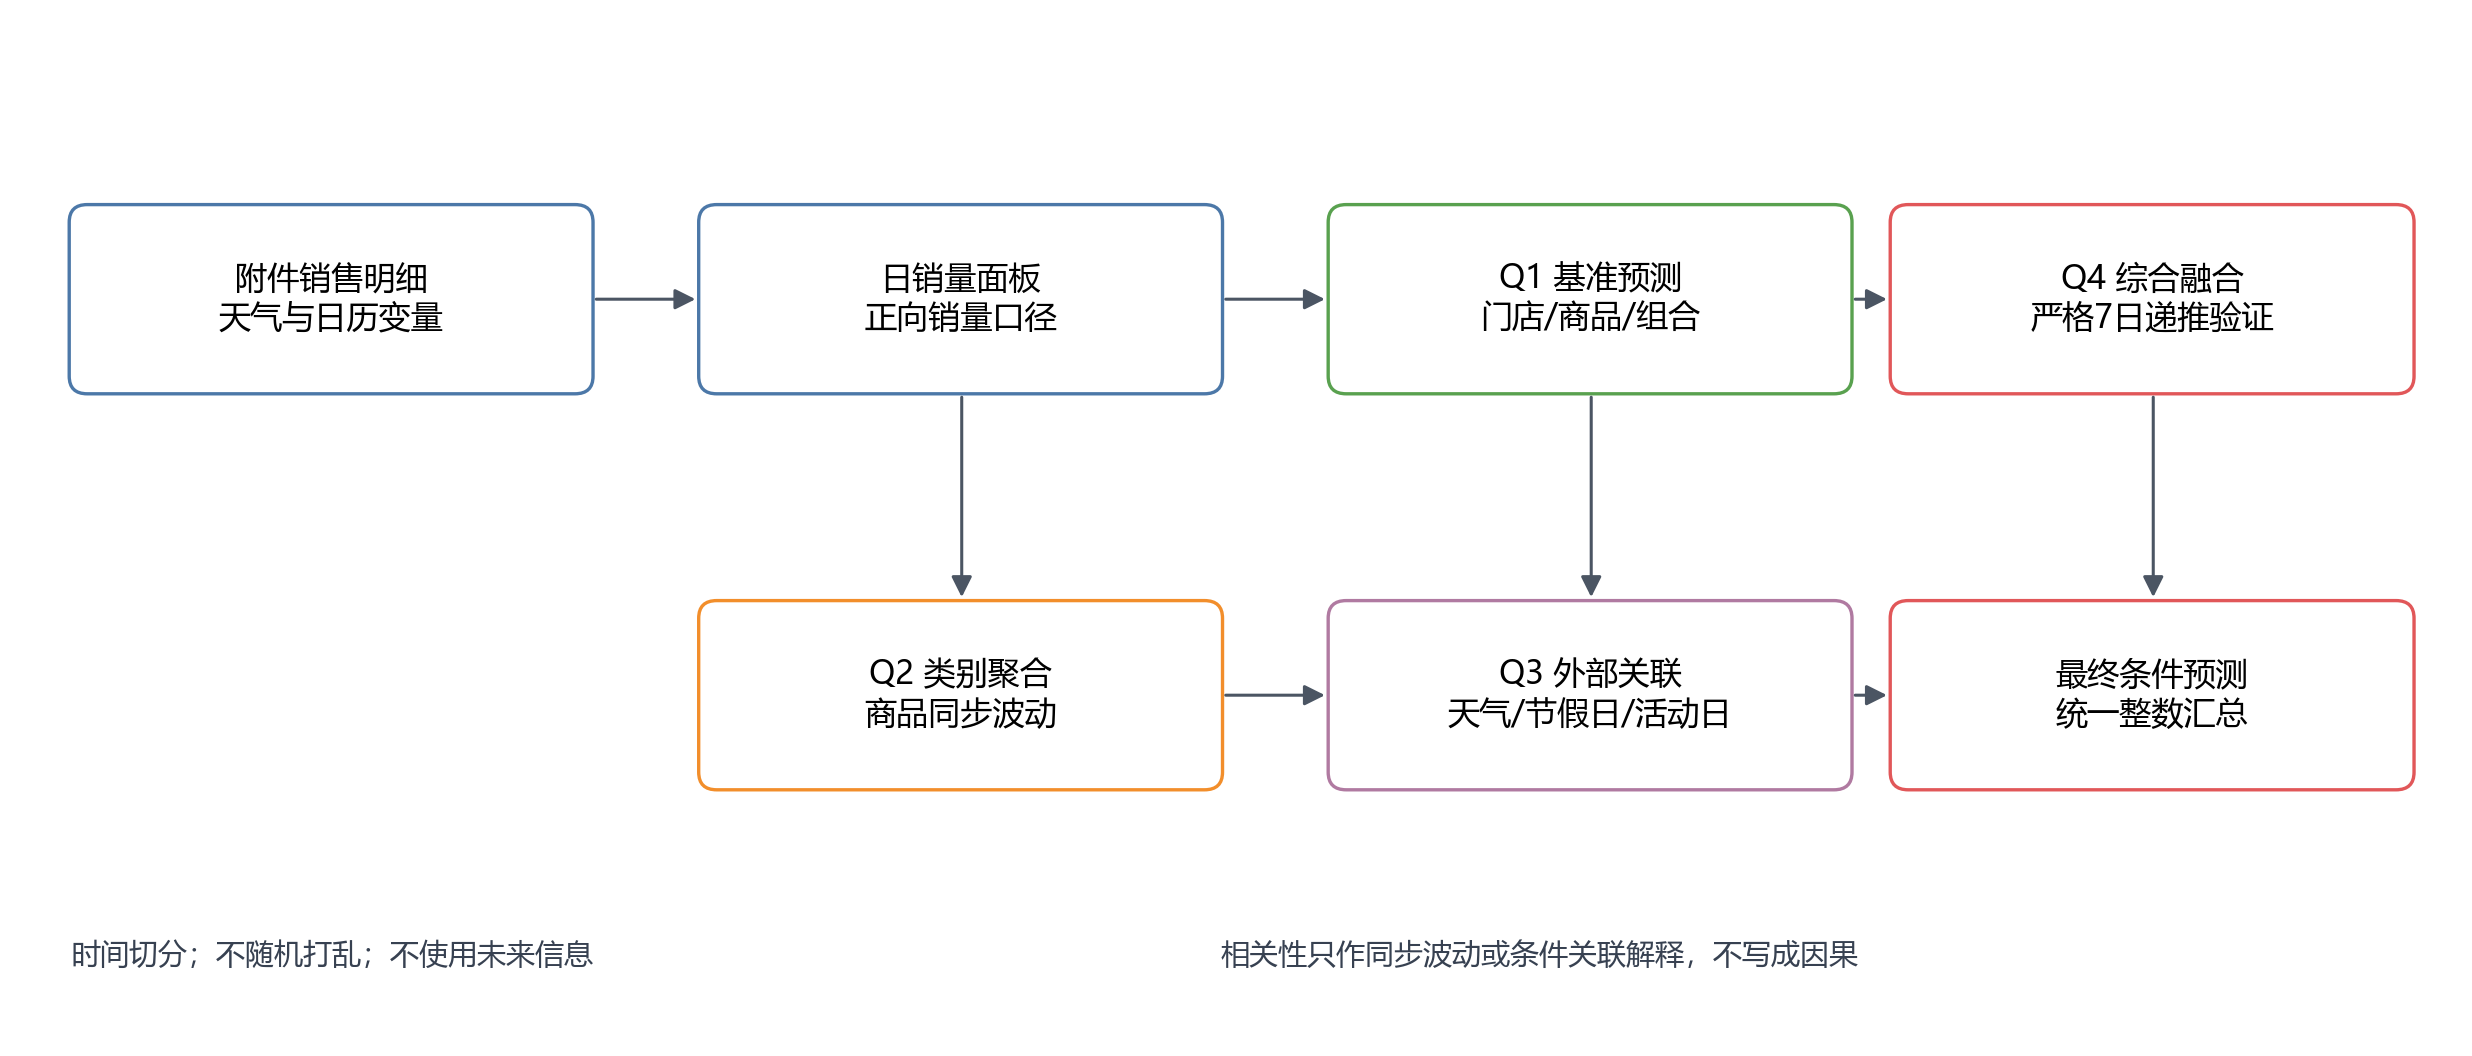
\includegraphics[width=0.95\textwidth]{technical_route_phase3.png}
\caption{四问关系与技术路线}
\label{fig:technical_route}
\end{figure}

预测评价不能随机切分，因为随机切分会让未来日期信息进入训练过程。本文使用时间顺序切分、日滚动验证和严格 7 日递推窗口验证。日滚动一步验证评价“每天更新真实销量后预测下一天”的能力；严格 7 日递推验证评价“窗口开始时一次性向未来预测 7 天”的能力，两者不能混用。

为避免不同章节的 WAPE 数值被误读，本文将三种验证口径统一列在表 \ref{tab:validation_modes}。全文以严格 7 日递推作为第四问和最终模型评价的主口径；日滚动一步和 7 日窗口总量验证只用于对应问题的方法筛选或补充复核。

\begin{table}[H]
\centering
\caption{三种验证口径的定义与适用范围}
\label{tab:validation_modes}
\resizebox{\textwidth}{!}{
\begin{tabular}{p{3.0cm}p{5.7cm}p{4.7cm}p{3.0cm}}
\toprule
验证口径 & 定义 & 适用范围 & 主要限制 \\
\midrule
日滚动一步验证 & 对验证期每一天，只使用该日期以前的真实历史销量预测当天；进入下一天时，前一天真实销量可作为历史信息更新。 & 问题一、问题二的基础模型筛选；问题三候选方法的预测参考。 & 更接近每日滚动运营，不等同于一次性预测未来 7 天。 \\
7 日窗口总量验证 & 将连续 7 天预测和真实销量分别汇总后计算误差，关注未来 7 天总量偏差。 & 问题一方法复核和聚合层运营可用性说明。 & 汇总会抵消部分日内误差，不能替代细粒度逐日验证。 \\
严格 7 日递推验证 & 每个窗口只使用窗口起点以前的真实历史训练；窗口内第 2 至第 7 天的滞后和滚动特征由前序预测值递推生成。 & 问题四综合模型、显著性检验和最终模型评价主口径。 & 只有 4 个完整验证窗口，统计功效有限。 \\
\bottomrule
\end{tabular}
}
\end{table}

模型选择遵循三条原则：第一，所有结论来自附件数据或明确的模型计算；第二，优先使用本科数学建模竞赛中可解释、可复现、可写入论文的方法；第三，复杂模型只有在误差稳定下降且解释成本可控时才作为主方案。各问题的方法取舍均以相同时间顺序验证下的误差表现和题目解释需求共同决定。

\section{模型假设与符号说明}

\subsection{模型假设}

\begin{enumerate}
  \item 题目提供的销售明细和外部变量记录总体真实可靠。对于已发现的数据问题，本文采用记录、标记和统一口径处理，而不是直接删除原始数据。
  \item 短期内历史销售规律具有一定延续性。未来 7 天预测依赖最近历史销量、同星期规律和类别/门店稳定差异。
  \item 负销量不代表顾客正常购买需求。根据人工确认，负销量多对应破损、过期或冲销类负向调整，因此预测目标采用正向销量。
  \item 附件类别字段可以作为同类零食的正式聚合依据。相关性聚类和销量规模分组只作为补充分析，不替代业务类别。
  \item 天气、节假日和活动日与销量之间可以存在统计关联，但当前数据不足以识别严格因果效应。本文所称“影响因素分析”均指统计关联分析。
  \item 未来 7 天无附件真实天气和真实活动安排。最终预测若使用天气和活动变量，应解释为“给定历史同期外部变量情景下”的条件预测。
\end{enumerate}

\subsection{符号说明}

\begin{table}[H]
\centering
\caption{主要符号说明}
\label{tab:symbols}
\begin{tabular}{ll}
\toprule
符号 & 含义 \\
\midrule
$t$ & 日期序号 \\
$s$ & 门店编号 \\
$p$ & 商品编号 \\
$g$ & 商品类别 \\
$y_{s,p,t}$ & 门店 $s$、商品 $p$ 在日期 $t$ 的正向销量 \\
$\hat y_{s,p,t}$ & 对 $y_{s,p,t}$ 的预测值 \\
$Y_{t,g}$ & 日期 $t$ 类别 $g$ 的聚合销量 \\
$S_t$ & 指数平滑中的平滑水平 \\
$\alpha$ & 指数平滑系数 \\
$r_{pq}$ & 商品 $p$ 与商品 $q$ 的销量相关系数 \\
$X_t$ & 日历、天气、活动日等外部变量 \\
$MAE$ & 平均绝对误差 \\
$RMSE$ & 均方根误差 \\
$WAPE$ & 加权绝对百分比误差 \\
\bottomrule
\end{tabular}
\end{table}

\section{数据预处理}
\label{sec:data_preprocessing}

\subsection{数据检查}

销售数据日期范围为 2020-04-01 至 2022-03-31，含 7 家门店、12 个商品代码、13 个商品名称和 8 个类别。商品代码 11001020 对应两个海苔商品名称，经人工确认以商品编号为准，名称差异视为录入笔误。天气数据日期范围为 2020-03-01 至 2022-03-30，不能覆盖销售最后一天 2022-03-31 和未来 2022-04-01 至 2022-04-07。

数据质量检查发现：销售明细中完全重复行 16605 条，经人工确认保留；负销量记录 54 条，作为损耗/冲销类负向调整；交易级数量范围为 -24 至 2712，IQR 规则标记 5536 条交易级极端记录。本文不删除原始记录，而是在处理表中保留正向销量、负向调整和异常标记。主要字段和处理口径见附录 A。

\subsection{日销量面板构造}

本文将交易明细聚合为日期--门店--商品日销量面板，并补齐出现过的门店--商品组合在完整日期上的零销量记录。处理后的日销量面板含 59130 行，日期范围为 2020-04-01 至 2022-03-31；合并外部变量后的建模表同样为 59130 行。

日销量字段包括：
\begin{itemize}
  \item \texttt{daily\_sales}：日净销量，包含负向调整；
  \item \texttt{positive\_sales}：正向销售数量，作为主预测目标；
  \item \texttt{negative\_adjustment\_qty}：负向调整数量绝对值；
  \item \texttt{has\_external\_data}：是否成功匹配附件二外部变量。
\end{itemize}

\subsection{外部变量处理}

附件二的“温度”和“温度.1”经人工确认为最高温和最低温，分别记为 \texttt{max\_temperature} 和 \texttt{min\_temperature}；“活动日”确认为门店促销活动日；“工休日”表示周末/节假日等休息日。附件二未提供湿度字段，因此本文不单独讨论湿度。缺少外部变量的销售日期为 2022-03-31，对应合并后 81 行 \texttt{has\_external\_data=0}。未来 7 天没有附件真实天气和活动日观测，本文在问题四中采用历史同期情景，并明确其条件预测性质。

\section{问题一：门店与商品销量分析及未来 7 天预测}

问题一以正向销量为目标，分别在门店、商品和门店--商品层级建模。设某一序列第 $t$ 天销量为 $y_t$。

\subsection{模型建立}

7 日移动平均模型为
\begin{equation}
\hat y_{t+1}=\frac{1}{7}\sum_{i=0}^{6}y_{t-i}.
\end{equation}
该模型用最近 7 天平均销量代表短期水平，适合作为门店层面的主模型。

同星期均值模型为
\begin{equation}
\hat y_t=\frac{1}{m}\sum_{j=1}^{m}y_{t-7j},\quad m\le 8.
\end{equation}
该模型用历史相同星期几销量预测目标日，作为检验星期效应的基准模型。

简单指数平滑模型为
\begin{equation}
S_t=\alpha y_t+(1-\alpha)S_{t-1},\quad \hat y_{t+1}=S_t,\quad 0<\alpha\le 1.
\end{equation}
该模型更重视近期销量，适合作为商品和门店--商品层面的主模型 \cite{hyndman2021fpp3}。

\subsection{验证结果}

阶段 2 日滚动验证结果见表 \ref{tab:q1_metrics}。

\begin{table}[H]
\centering
\caption{问题一日滚动验证下主模型误差}
\label{tab:q1_metrics}
\begin{tabular}{llrrr}
\toprule
层级 & 主模型 & MAE & RMSE & WAPE \\
\midrule
门店 & 移动平均(7日) & 9.685 & 15.445 & 37.49\% \\
商品 & 简单指数平滑 & 5.748 & 10.968 & 38.14\% \\
门店--商品 & 简单指数平滑 & 1.783 & 3.733 & 74.95\% \\
\bottomrule
\end{tabular}
\end{table}

为了使评价更贴近“未来 7 天总销量”，方法复核中补充 7 日窗口总量验证。结果显示，原问题一主方案在商品层面 WAPE=21.51\%，门店层面 WAPE=22.12\%，门店--商品层面 WAPE=43.06\%。更复杂的滞后 Ridge 和随机森林未形成稳定优势，因此问题一保留原主模型。

\subsection{描述性图表}

\begin{figure}[H]
\centering
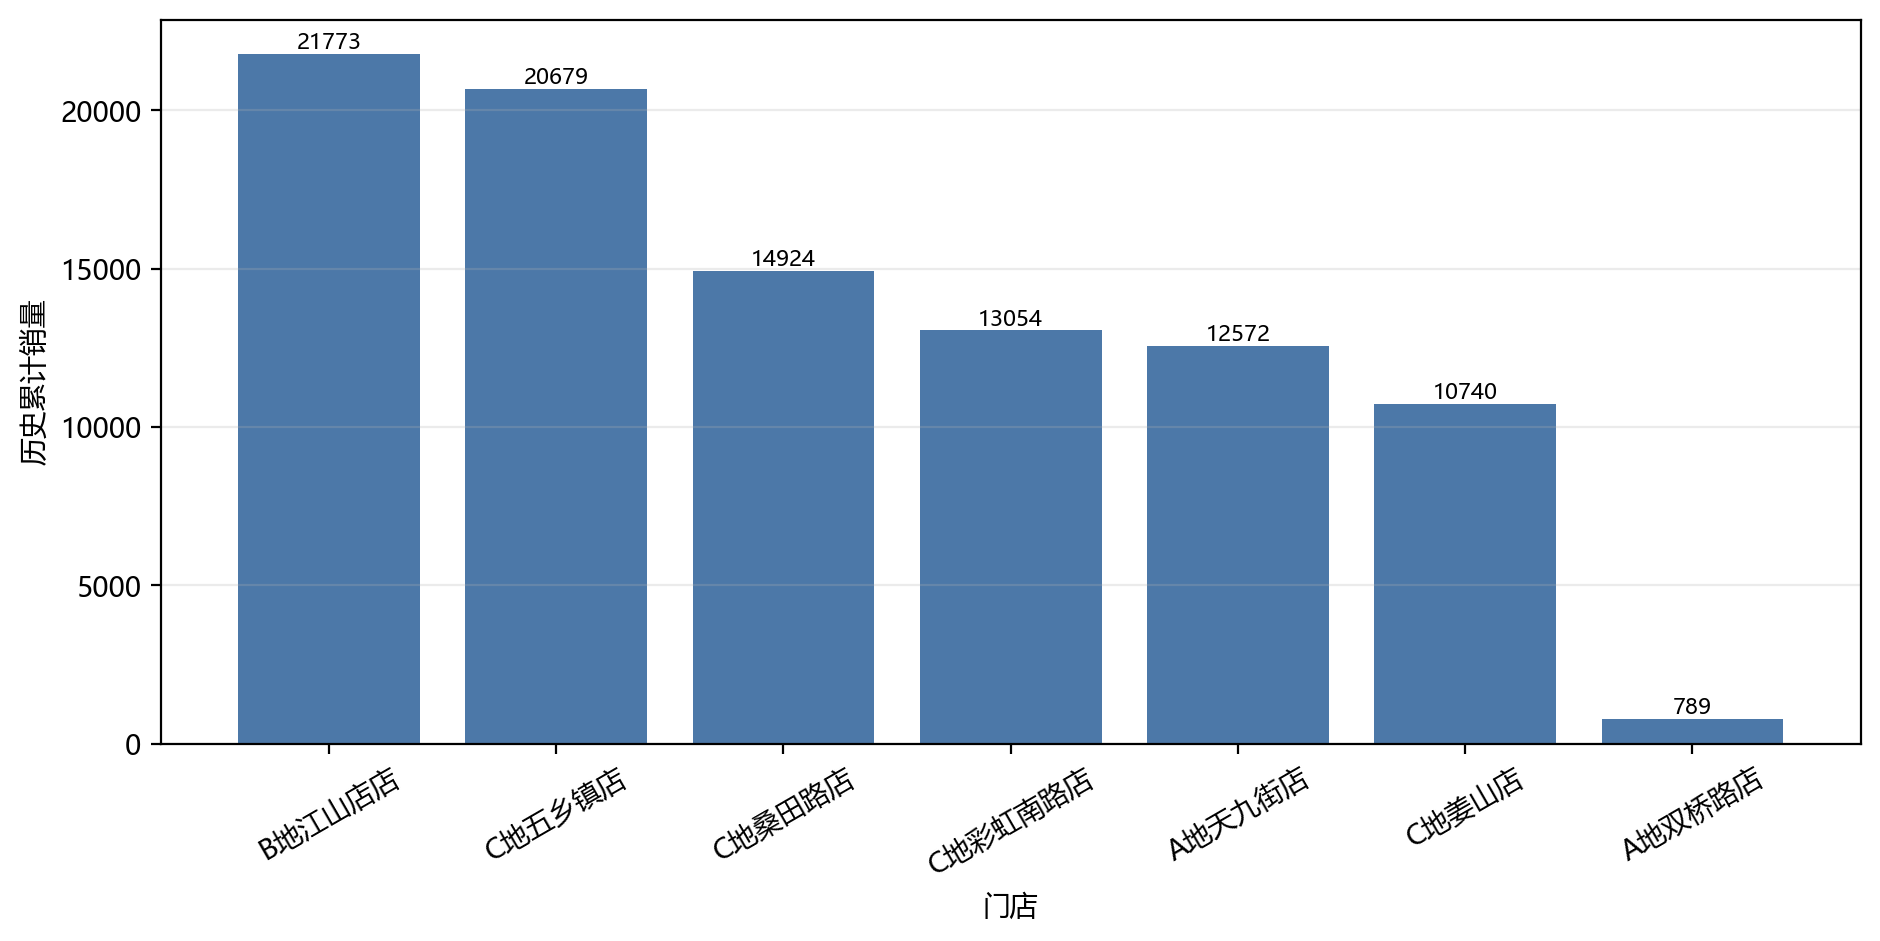
\includegraphics[width=0.88\textwidth]{q1_store_total_sales.png}
\caption{各门店历史累计销量}
\label{fig:q1_store_total}
\end{figure}

\begin{figure}[H]
\centering
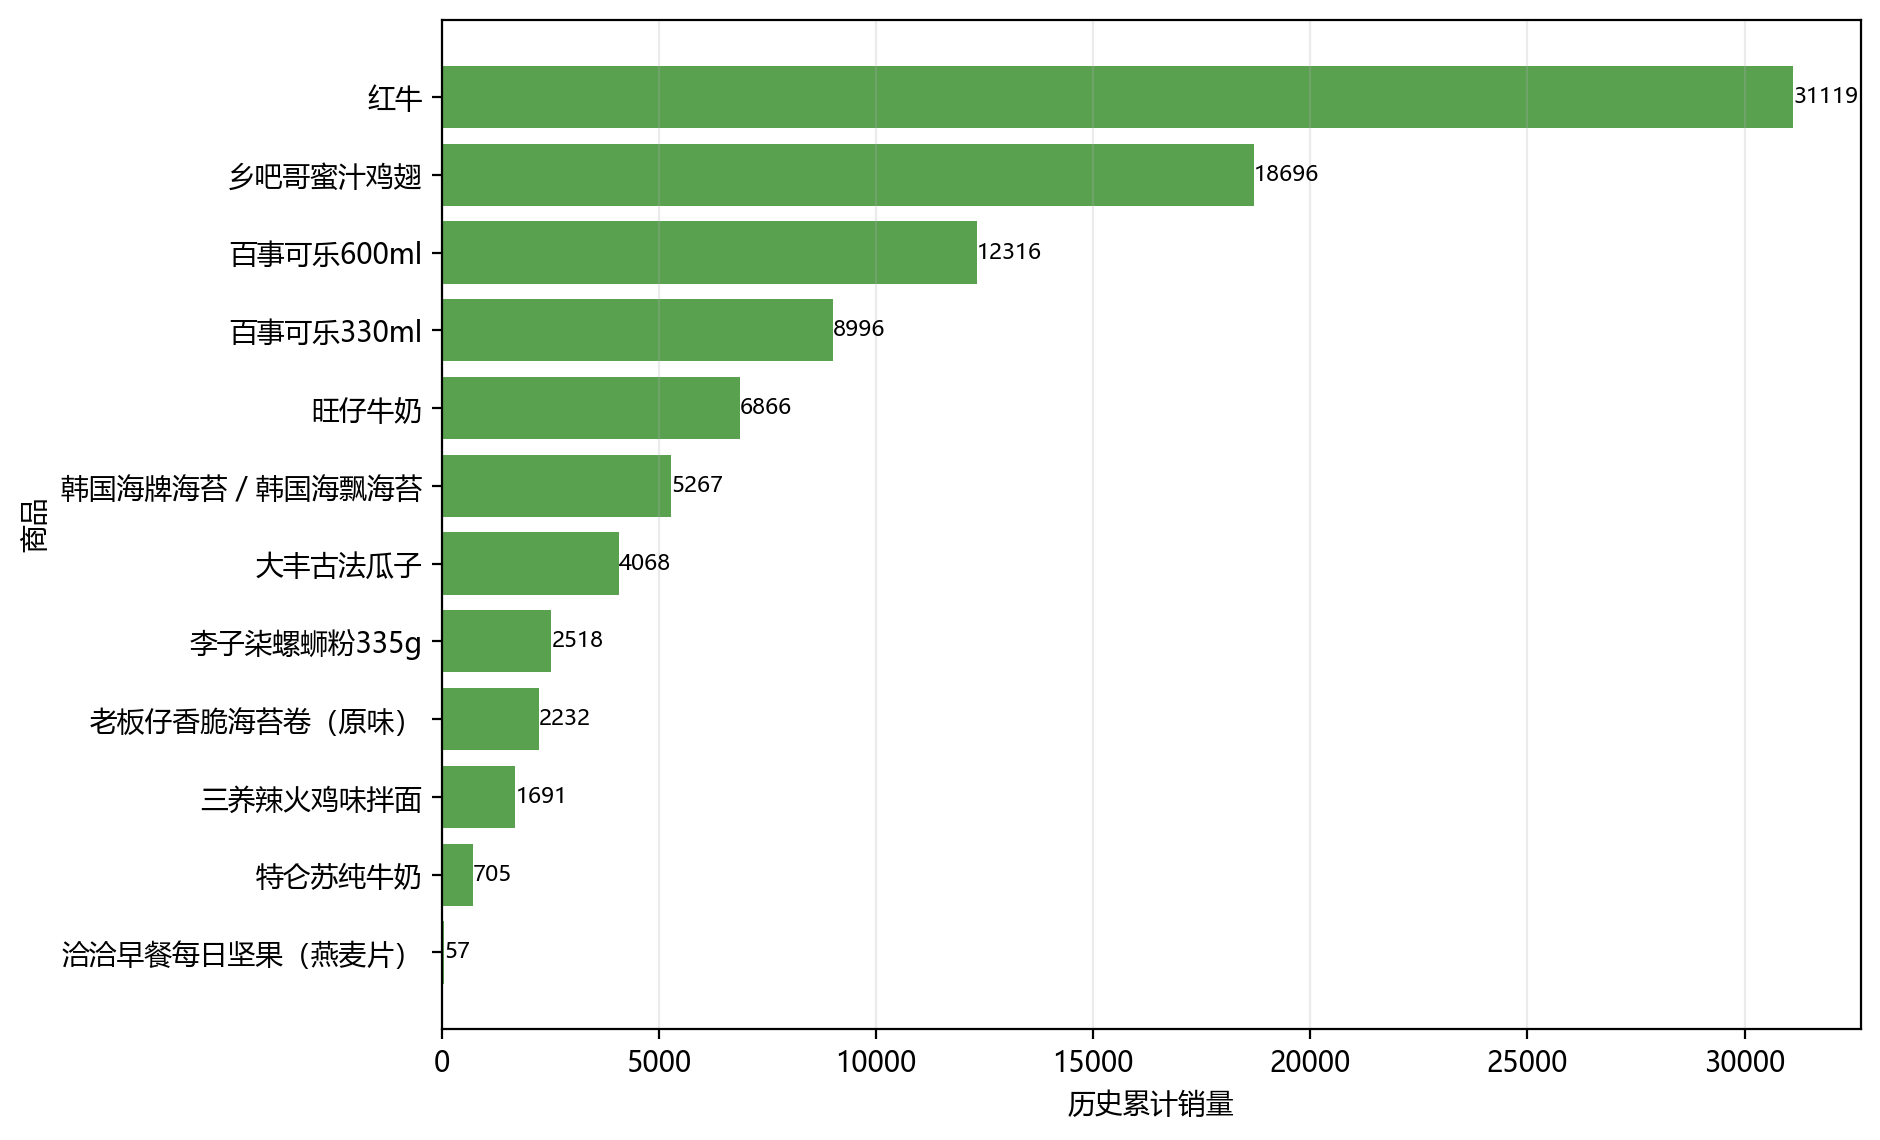
\includegraphics[width=0.88\textwidth]{q1_product_total_sales.png}
\caption{各商品历史累计销量}
\label{fig:q1_product_total}
\end{figure}

\begin{figure}[H]
\centering
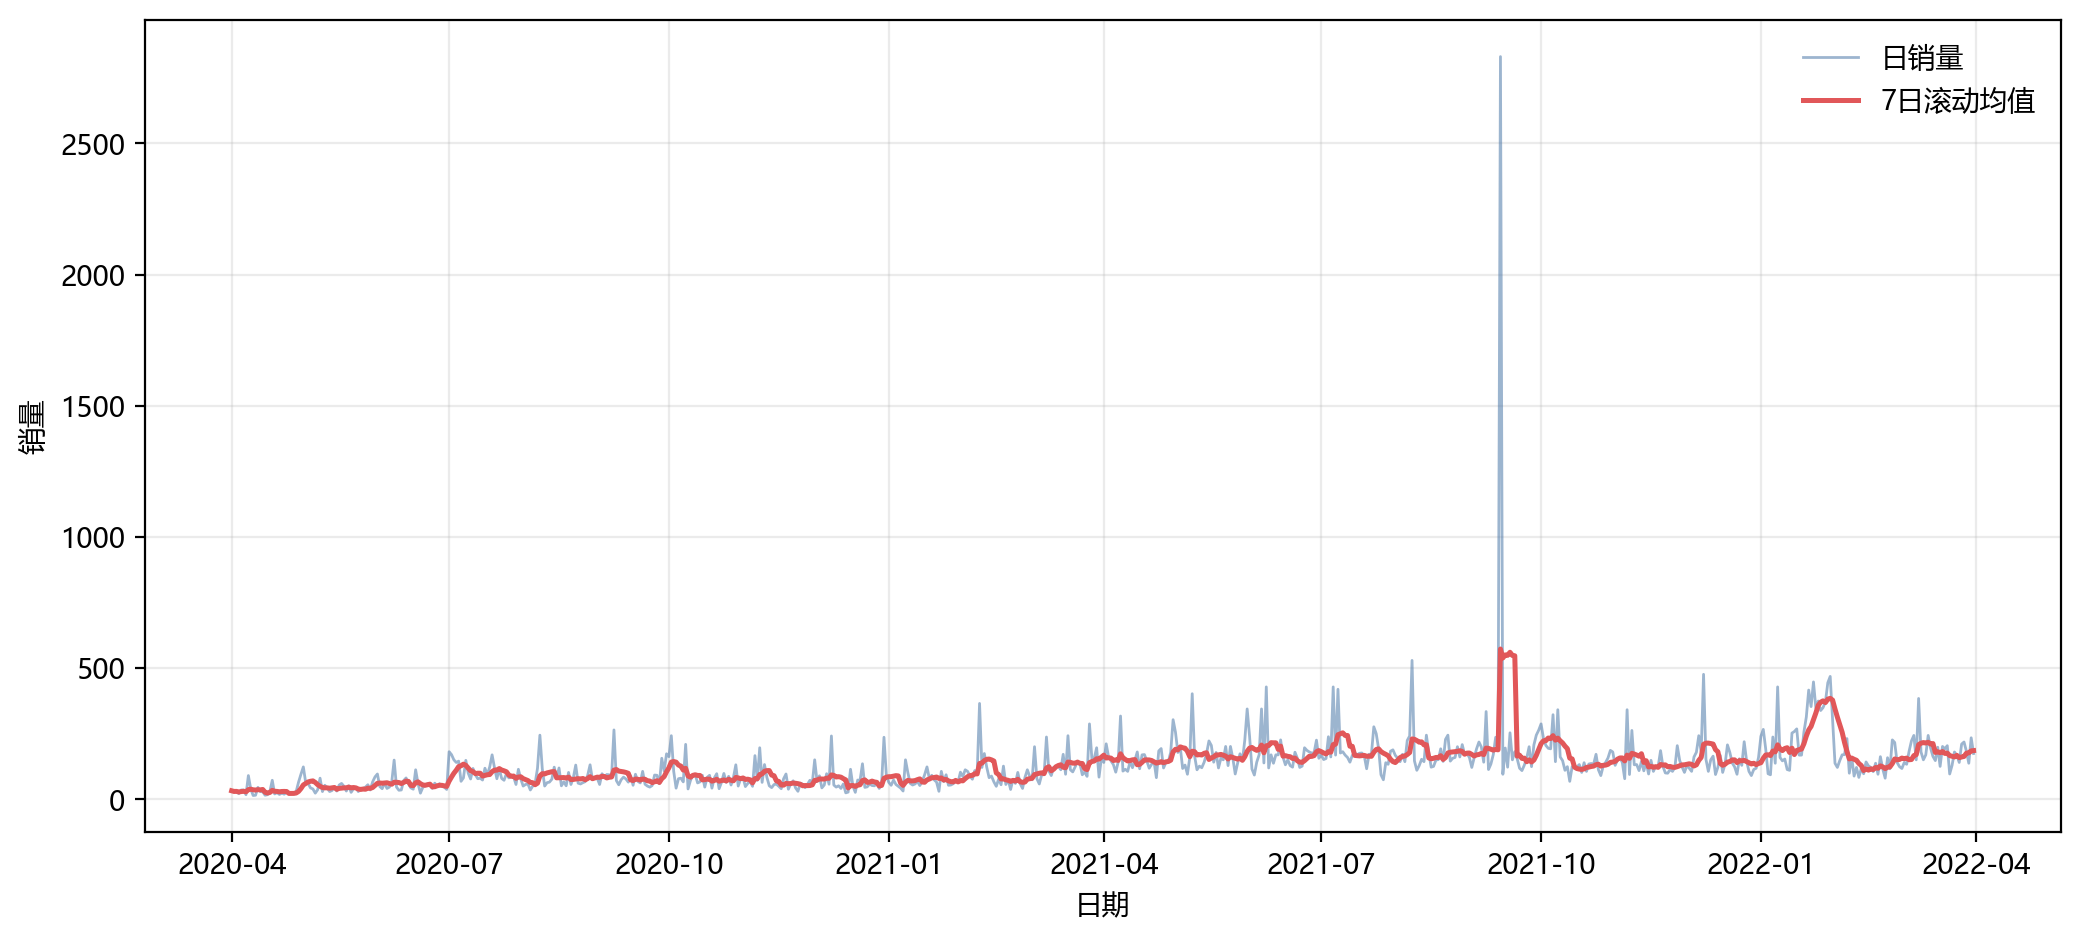
\includegraphics[width=0.92\textwidth]{q1_daily_total_trend.png}
\caption{总体日销量历史趋势}
\label{fig:q1_daily_trend}
\end{figure}

\begin{figure}[H]
\centering
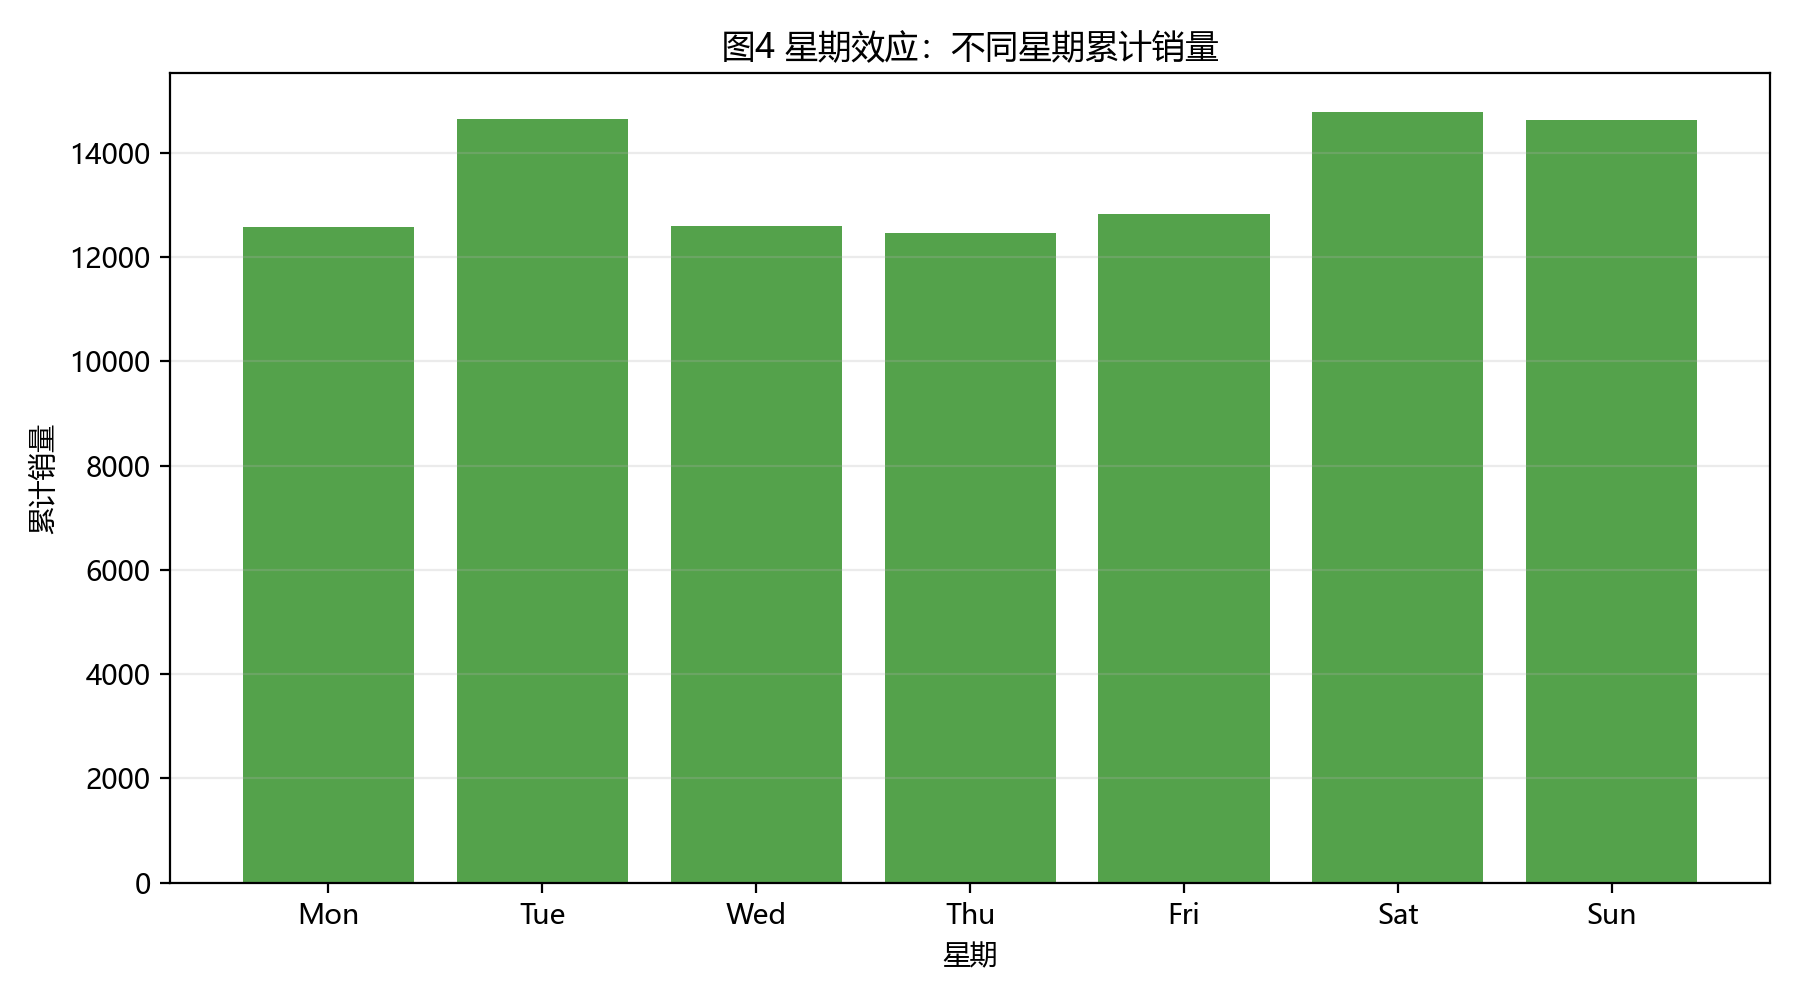
\includegraphics[width=0.82\textwidth]{q1_weekday_effect.png}
\caption{不同星期的平均销量}
\label{fig:q1_weekday}
\end{figure}

\begin{figure}[H]
\centering
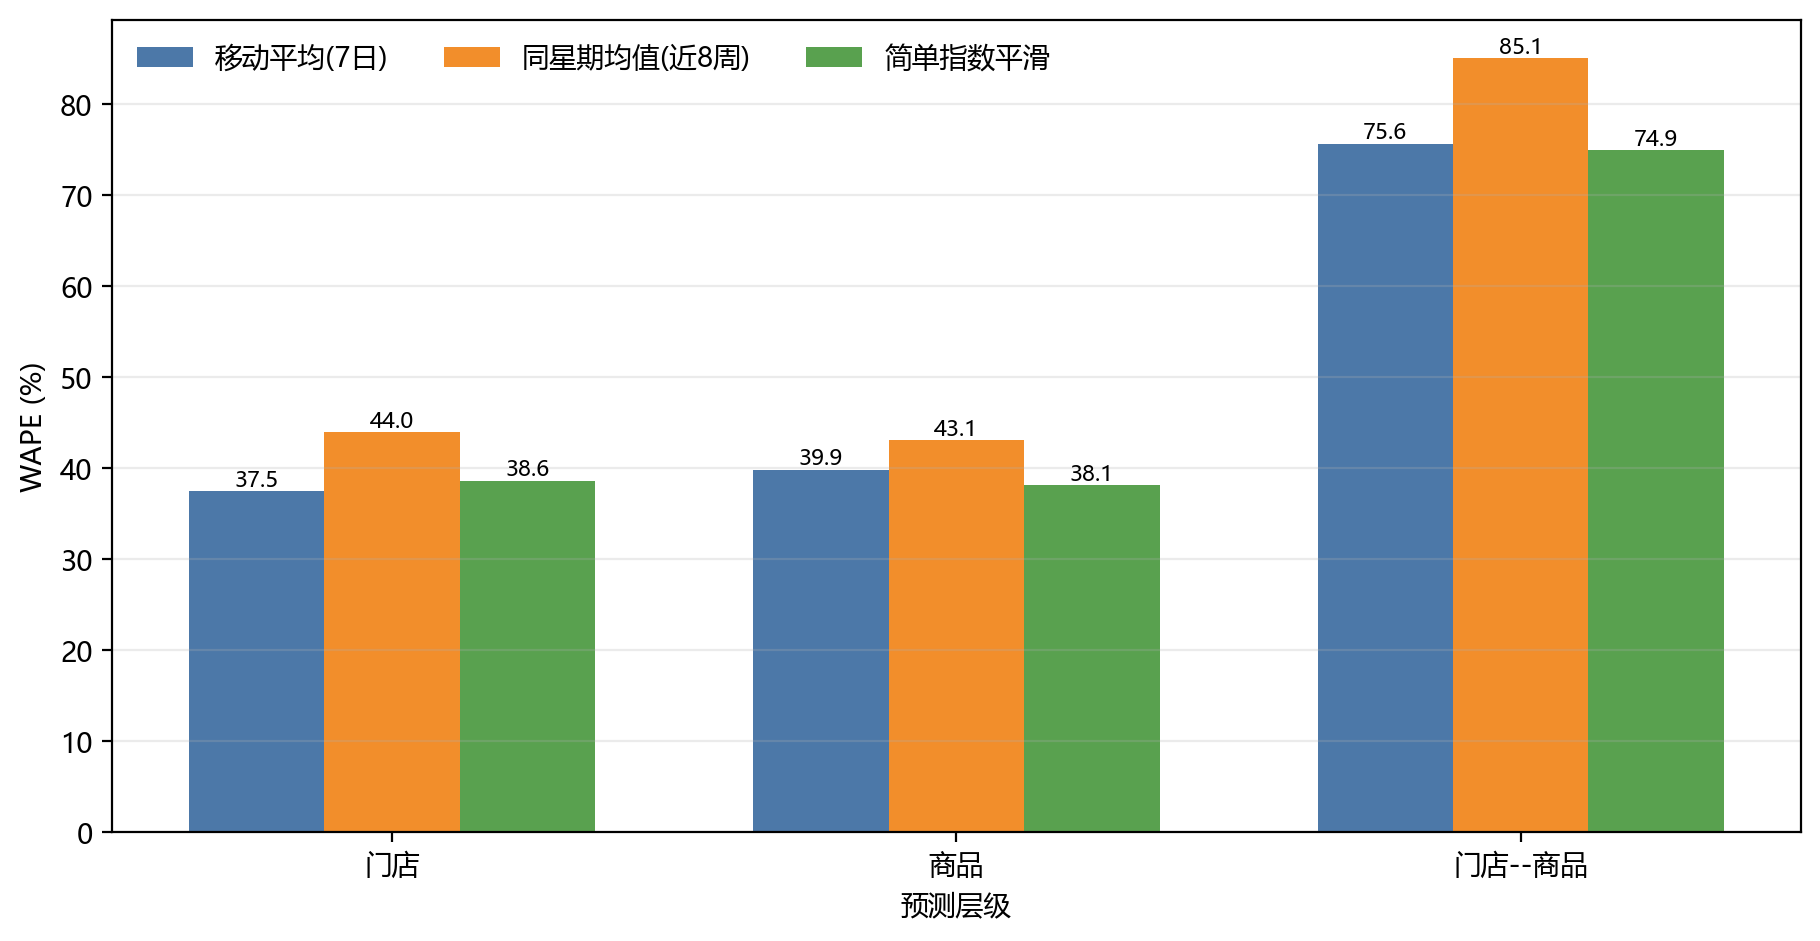
\includegraphics[width=0.82\textwidth]{q1_model_wape_comparison.png}
\caption{问题一各层级模型 WAPE 对比}
\label{fig:q1_wape}
\end{figure}

\subsection{问题一结果}

历史累计销量最高的门店为 B地江山店店，累计销量 21773；历史累计销量最高的商品为红牛，累计销量 31119。门店和商品销量规模差异明显，说明不能只用统一平均水平预测所有对象。

未来 7 天门店预测中，B地江山店店预测总销量最高，为 309.0；C地五乡镇店为 280.0；A地天九街店为 245.0。商品预测中，乡吧哥蜜汁鸡翅预测 389.613，红牛预测 286.719，百事可乐600ml 预测 136.219。问题一门店层面和商品层面分别建模，预测总量没有强制一致：门店层面合计 1296.000，商品层面合计 1226.006。

\section{问题二：商品关联分析与类别聚合预测}

问题二关注同一门店中不同零食销量之间的联系，并要求整合同类零食预测未来 7 天总销量。设 $y_{t,p}$ 表示第 $t$ 天商品 $p$ 的正向销量，$c(p)$ 表示商品所属类别。

\subsection{商品销量矩阵与相关性}

对每个门店构造日期 $\times$ 商品销量矩阵：
\begin{equation}
Y_s=(y_{t,p}),\quad t=1,\ldots,n,\ p=1,\ldots,m.
\end{equation}
商品 $p$ 与商品 $q$ 的 Pearson 相关系数为
\begin{equation}
r_{pq}=
\frac{\sum_t(y_{t,p}-\bar y_p)(y_{t,q}-\bar y_q)}
{\sqrt{\sum_t(y_{t,p}-\bar y_p)^2}\sqrt{\sum_t(y_{t,q}-\bar y_q)^2}}.
\end{equation}
为避免单一 Pearson 相关造成过度解释，本文补充 Spearman 相关、去星期效应 Pearson 和门店内相关稳定性检查。商品关联结论只解释为同步波动，不写成因果或替代关系。

\begin{figure}[H]
\centering
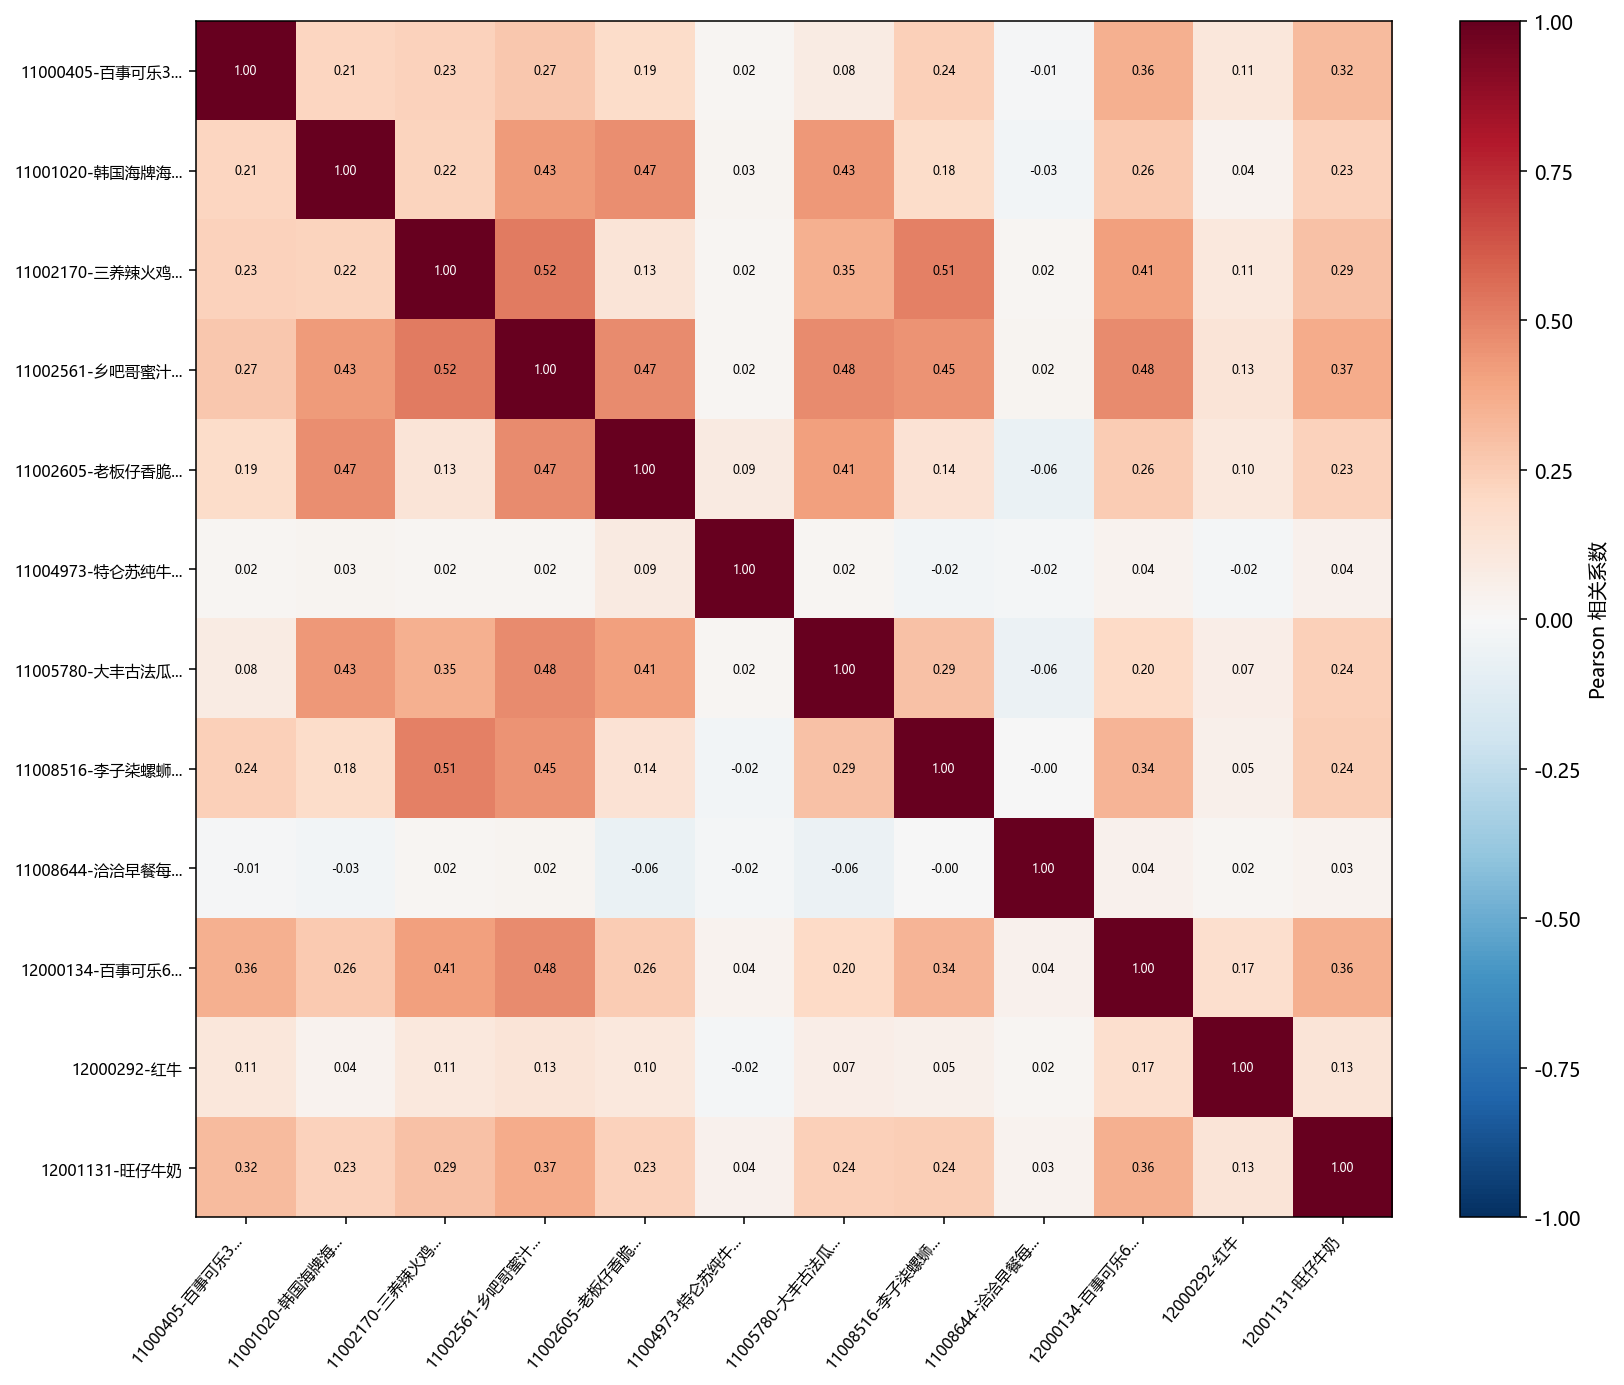
\includegraphics[width=0.95\textwidth]{q2_overall_product_correlation_heatmap.png}
\caption{商品日销量相关性热力图}
\label{fig:q2_corr}
\end{figure}

全部门店汇总层面共计算 $12$ 个商品代码之间的 66 对 Pearson 相关系数。本文将 $r\ge 0.50$ 记为强正相关，将 $|r|\le 0.10$ 记为弱线性相关。结果中有 2 对强正相关商品对，见表 \ref{tab:q2_strong_pairs}；有 25 对弱相关商品对，见表 \ref{tab:q2_weak_pairs}。

\begin{table}[H]
\centering
\caption{强正相关商品对}
\label{tab:q2_strong_pairs}
\begin{tabular}{llrr}
\toprule
商品 A & 商品 B & 相关系数 & 同日均有销量天数 \\
\midrule
三养辣火鸡味拌面 & 乡吧哥蜜汁鸡翅 & 0.521 & 516 \\
三养辣火鸡味拌面 & 李子柒螺蛳粉335g & 0.506 & 400 \\
\bottomrule
\end{tabular}
\end{table}

\begingroup
\small
\setlength{\tabcolsep}{4pt}
\begin{longtable}{p{4.4cm}p{4.6cm}p{1.7cm}p{2.0cm}}
\caption{弱相关商品对（$|r|\le 0.10$）}
\label{tab:q2_weak_pairs}\\
\toprule
商品 A & 商品 B & 相关系数 & 同日均有销量天数 \\
\midrule
\endfirsthead
\toprule
商品 A & 商品 B & 相关系数 & 同日均有销量天数 \\
\midrule
\endhead
老板仔香脆海苔卷（原味） & 洽洽早餐每日坚果（燕麦片） & -0.063 & 11 \\
大丰古法瓜子 & 洽洽早餐每日坚果（燕麦片） & -0.055 & 16 \\
韩国海牌海苔 / 韩国海飘海苔 & 洽洽早餐每日坚果（燕麦片） & -0.026 & 17 \\
特仑苏纯牛奶 & 李子柒螺蛳粉335g & -0.025 & 254 \\
特仑苏纯牛奶 & 红牛 & -0.018 & 390 \\
特仑苏纯牛奶 & 洽洽早餐每日坚果（燕麦片） & -0.016 & 9 \\
百事可乐330ml & 洽洽早餐每日坚果（燕麦片） & -0.009 & 17 \\
李子柒螺蛳粉335g & 洽洽早餐每日坚果（燕麦片） & -0.004 & 16 \\
洽洽早餐每日坚果（燕麦片） & 红牛 & 0.018 & 17 \\
三养辣火鸡味拌面 & 洽洽早餐每日坚果（燕麦片） & 0.019 & 14 \\
百事可乐330ml & 特仑苏纯牛奶 & 0.020 & 375 \\
乡吧哥蜜汁鸡翅 & 特仑苏纯牛奶 & 0.020 & 380 \\
特仑苏纯牛奶 & 大丰古法瓜子 & 0.020 & 377 \\
三养辣火鸡味拌面 & 特仑苏纯牛奶 & 0.023 & 288 \\
乡吧哥蜜汁鸡翅 & 洽洽早餐每日坚果（燕麦片） & 0.024 & 17 \\
韩国海牌海苔 / 韩国海飘海苔 & 特仑苏纯牛奶 & 0.028 & 374 \\
洽洽早餐每日坚果（燕麦片） & 旺仔牛奶 & 0.034 & 17 \\
特仑苏纯牛奶 & 百事可乐600ml & 0.036 & 391 \\
韩国海牌海苔 / 韩国海飘海苔 & 红牛 & 0.037 & 699 \\
洽洽早餐每日坚果（燕麦片） & 百事可乐600ml & 0.041 & 17 \\
特仑苏纯牛奶 & 旺仔牛奶 & 0.045 & 368 \\
李子柒螺蛳粉335g & 红牛 & 0.054 & 491 \\
大丰古法瓜子 & 红牛 & 0.065 & 699 \\
百事可乐330ml & 大丰古法瓜子 & 0.085 & 679 \\
老板仔香脆海苔卷（原味） & 特仑苏纯牛奶 & 0.091 & 301 \\
\bottomrule
\end{longtable}
\endgroup

表 \ref{tab:q2_strong_pairs} 中两对强正相关都包含三养辣火鸡味拌面，更合理的解释是它们在历史日销量上同步波动，可能共同受到客流、即时餐食消费场景或促销陈列节奏影响。表 \ref{tab:q2_weak_pairs} 中，多数弱相关对涉及低销量商品或消费场景差异较大的商品；这说明在当前附件数据下，不能把相关性弱或略为负相关直接解释为替代关系。

\subsection{同类零食整合}

类别聚合按附件 \texttt{category} 字段进行：
\begin{equation}
Y_{t,g}=\sum_{p:c(p)=g}y_{t,p}.
\end{equation}
该字段具有业务含义，因此作为“同类零食”的正式聚合依据。相关性聚类和销量规模分组可作为补充探索，但不替代附件业务类别。

\begin{figure}[H]
\centering
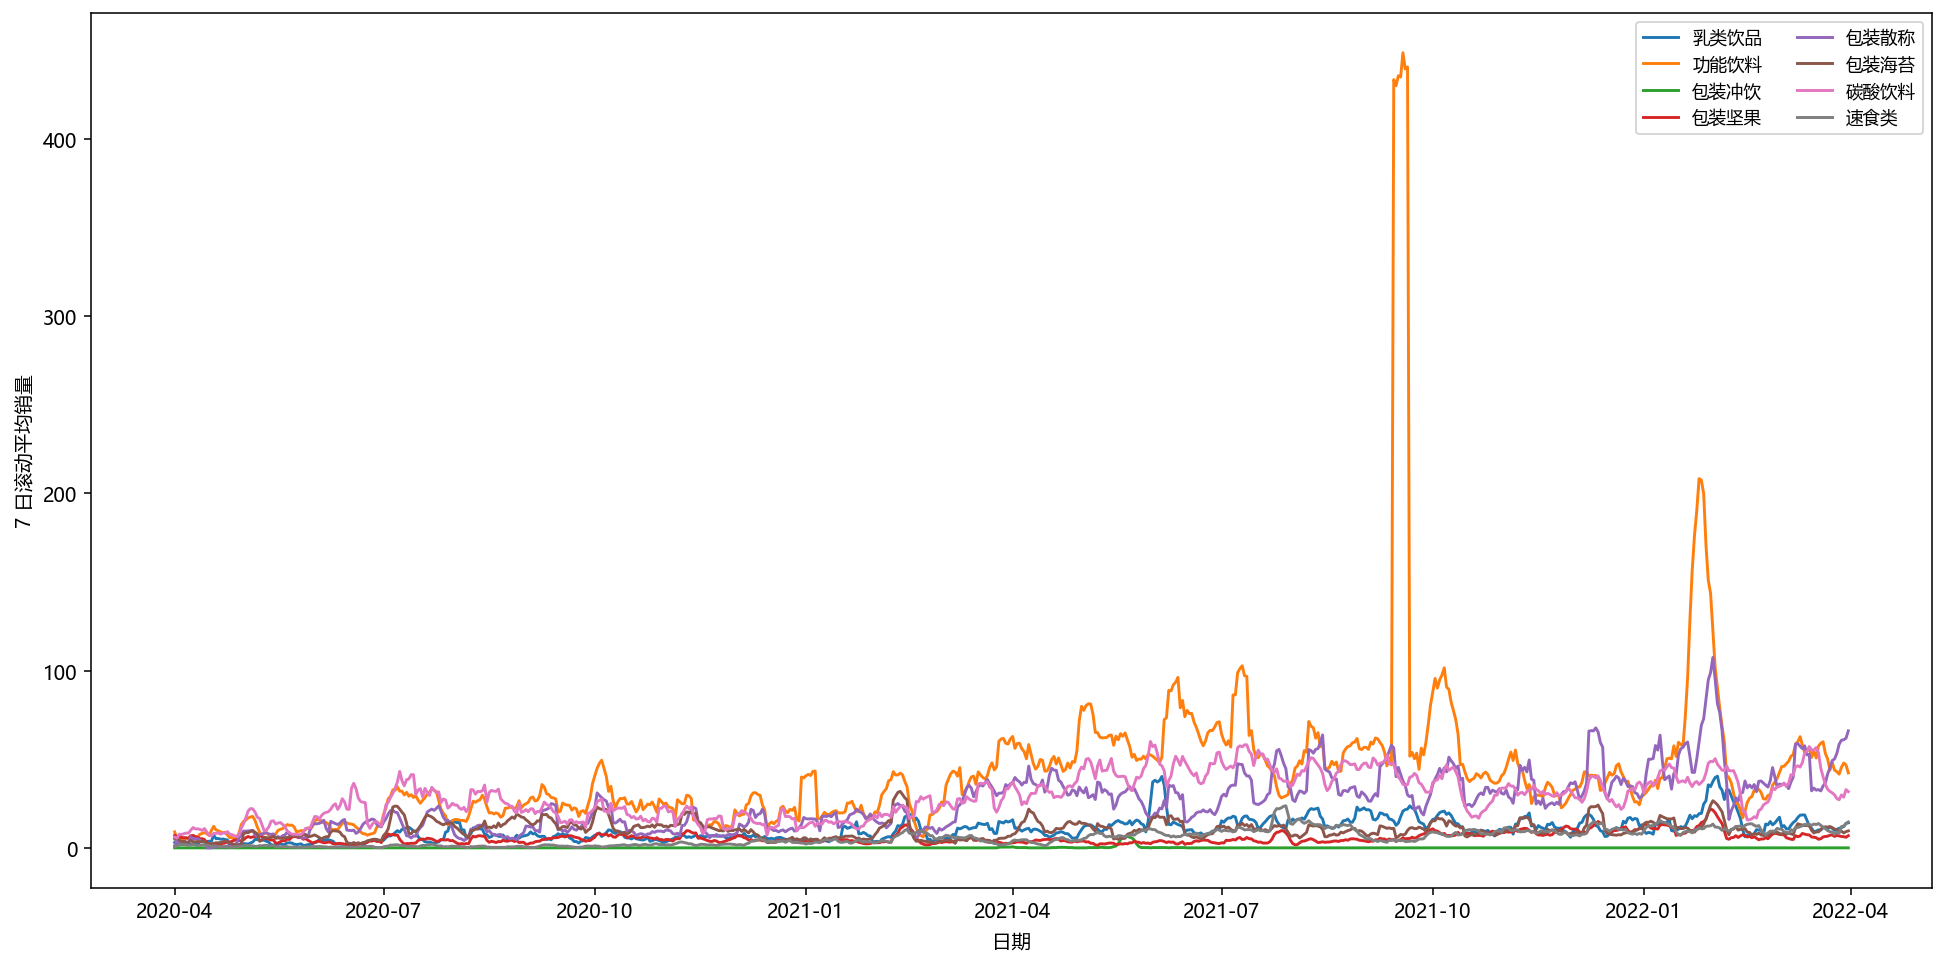
\includegraphics[width=0.94\textwidth]{q2_category_daily_trend.png}
\caption{各类别日销量历史趋势}
\label{fig:q2_category_trend}
\end{figure}

\subsection{类别预测与误差比较}

本文比较“单品预测后按类别加总”和“类别聚合后直接预测”。验证结果见表 \ref{tab:q2_metrics}，口径为 2022 年 3 月日滚动一步验证。

\begin{table}[H]
\centering
\caption{问题二类别预测策略误差比较（日滚动一步验证）}
\label{tab:q2_metrics}
\begin{tabular}{llrrr}
\toprule
方法 & 模型 & MAE & RMSE & WAPE \\
\midrule
类别聚合后直接预测 & 简单指数平滑 & 7.853 & 13.933 & 34.74\% \\
单品预测后按类别加总 & 简单指数平滑 & 7.873 & 13.949 & 34.83\% \\
类别聚合后直接预测 & 移动平均(7日) & 8.246 & 14.174 & 36.48\% \\
类别聚合后直接预测 & 同星期均值(近8周) & 8.851 & 15.057 & 39.15\% \\
\bottomrule
\end{tabular}
\end{table}

因此，问题二主方案采用“附件类别聚合后直接预测 + 简单指数平滑”。方法复核中，相关性聚类在同一日滚动一步验证下 WAPE=31.02\%，销量规模分组 WAPE=24.24\%，但前者业务类别含义弱，后者预测对象变成高/中/低销量组，均不替代附件类别主方案。

\subsection{问题二结果}

商品关联分析表明，全部门店汇总层面存在 2 对强正相关商品对和 25 对弱相关商品对。强正相关只能说明历史日销量同步波动，可能共同受客流、消费场景或促销节奏影响，不能证明商品之间存在直接带动关系。负相关候选的相关系数绝对值较小，当前数据未发现强替代关系证据。

类别预测结果显示，未来 7 天预测最高的类别为包装散称，预测 389.613；其次为功能饮料，预测 286.719；碳酸饮料预测 247.326。类别聚合可以降低单品零销量和偶然大单带来的波动，但会损失同一类别内部商品差异。

\section{问题三：外部因素统计关联分析}

问题三分析天气、节假日、活动日等外部因素与零食销量之间的统计关联。本文将外部因素构造为分类变量和连续变量：天气类型合并为更稳定的天气组，最高温、最低温、平均温度、昼夜温差和风力为连续变量，节假日、周末、活动日为 0--1 变量，星期、月份、门店、商品和历史销量作为控制变量。原始附件中没有湿度字段，因此不构造湿度变量。

\subsection{描述性分析}

对某一外部因素 $G$，先计算不同分组下的平均销量：
\begin{equation}
\bar y_g=\frac{1}{n_g}\sum_{i:G_i=g}y_i.
\end{equation}
该方法直观，但不能控制门店、商品和星期等混杂因素，只作为现象展示。

\begin{figure}[H]
\centering
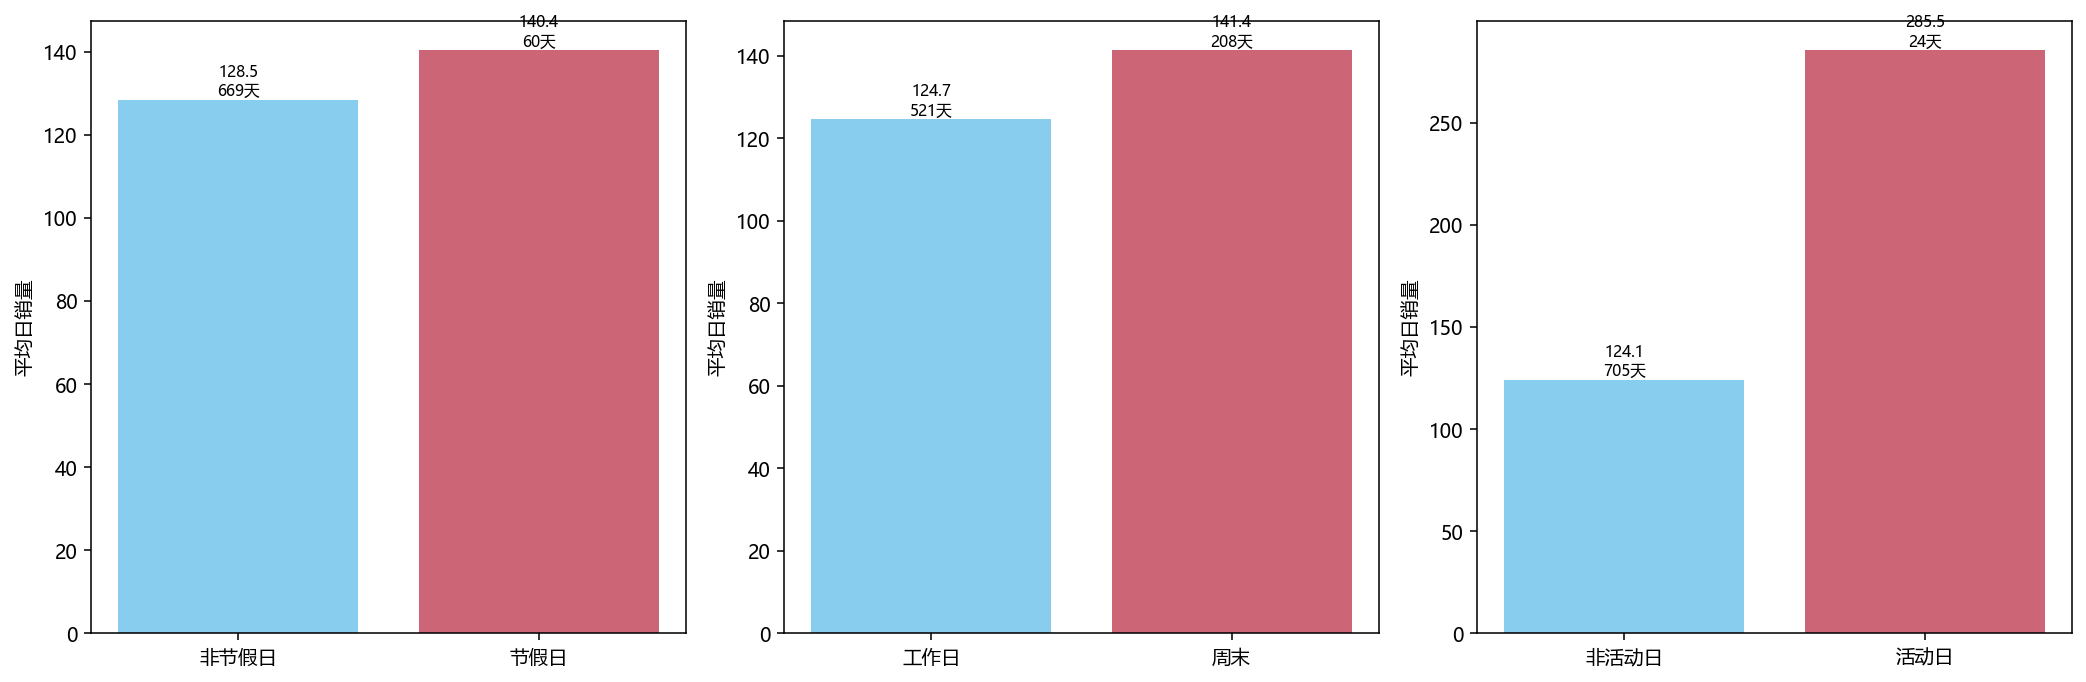
\includegraphics[width=0.85\textwidth]{q3_binary_factor_mean_sales.png}
\caption{二元外部因素均值差异，用于展示节假日、周末和活动日下的描述性销量差异}
\label{fig:q3_binary}
\end{figure}

\subsection{固定效应回归模型}

问题三主模型采用“合并天气 + 对数销量 + 历史控制固定效应回归”。设
$z_{s,p,t}=\log(1+y_{s,p,t})$，模型形式为
\begin{equation}
z_{s,p,t}=\beta_0+\beta^\top External_t+\rho_1 lag7_{s,p,t}
+\rho_2 rolling28_{s,p,t}+\gamma_s+\delta_p+\eta_w+\mu_m+\varepsilon_{s,p,t}.
\end{equation}
其中，$External_t$ 包括合并天气类别、平均温度、昼夜温差、风力、节假日和活动日；$\gamma_s$、$\delta_p$、$\eta_w$、$\mu_m$ 分别表示门店、商品、星期和月份固定效应；\texttt{lag\_7} 和 \texttt{rolling\_28\_prev} 只使用过去销量。线性回归和固定效应思想参考 \cite{montgomery2012regression}。

选择该模型的原因是：详细天气类别中存在雨夹雪、暴雨等少数样本天气，直接排序容易不稳；原始销量分布偏斜，对极端销量敏感；加入历史控制项后能减少基础需求差异对外部变量系数的干扰。

方法探索验证指标见表 \ref{tab:q3_methods}。

\begin{table}[H]
\centering
\caption{问题三外部因素分析方法验证指标}
\label{tab:q3_methods}
\resizebox{\textwidth}{!}{
\begin{tabular}{lrrrl}
\toprule
方法 & MAE & RMSE & WAPE & 论文定位 \\
\midrule
原方案详细天气 FE 回归 & 1.969 & 4.144 & 88.09\% & 补充 \\
合并天气 + 对数销量 + 历史控制 FE 回归 & 1.890 & 4.448 & 84.53\% & 主分析 \\
温度分箱 + 对数销量 + 历史控制 FE 回归 & 1.889 & 4.445 & 84.51\% & 非线性检查 \\
去异常日 + 对数销量 + 历史控制 FE 回归 & 1.825 & 4.254 & 84.94\% & 稳健性检查 \\
随机森林 grouped weather + history & 1.892 & 4.178 & 84.66\% & 预测贡献补充 \\
\bottomrule
\end{tabular}
}
\end{table}

\begin{figure}[H]
\centering
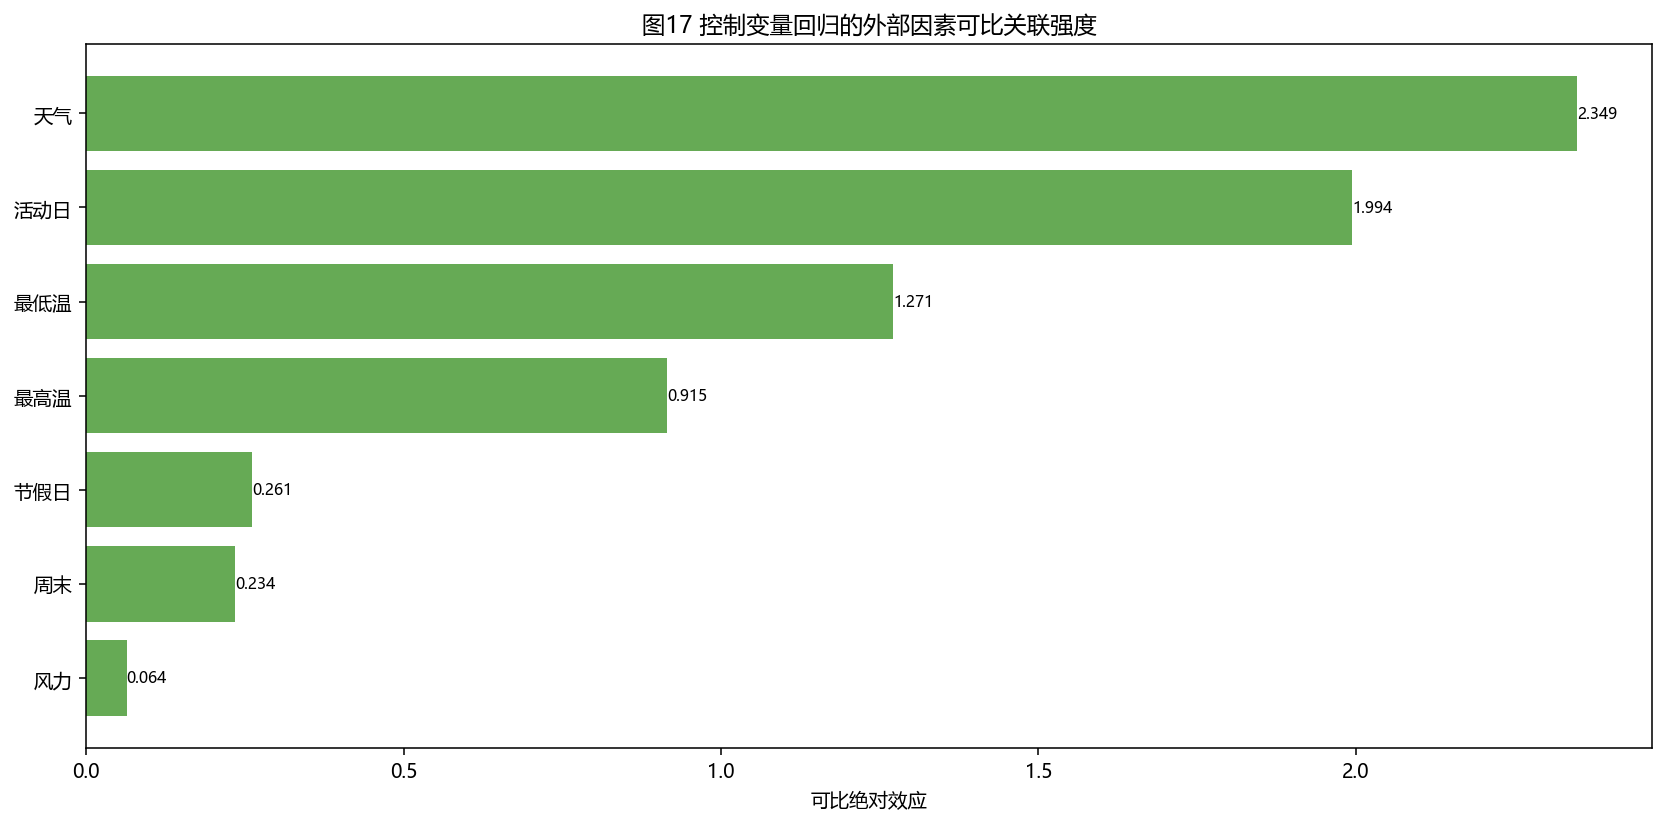
\includegraphics[width=0.86\textwidth]{q3_regression_factor_effect_ranking.png}
\caption{回归关联强度排序，用于展示外部变量在控制部分混杂因素后的可比统计关联}
\label{fig:q3_regression}
\end{figure}

\subsection{机器学习辅助分析}

随机森林置换重要性用于补充判断非线性预测贡献 \cite{breiman2001random}。它能说明打乱某一特征后预测误差增加多少，但不能说明销量变化方向，也不能证明因果关系。因此，问题三最终结论以回归的统计关联方向为主，以随机森林重要性作为辅助排序依据。

\begin{figure}[H]
\centering
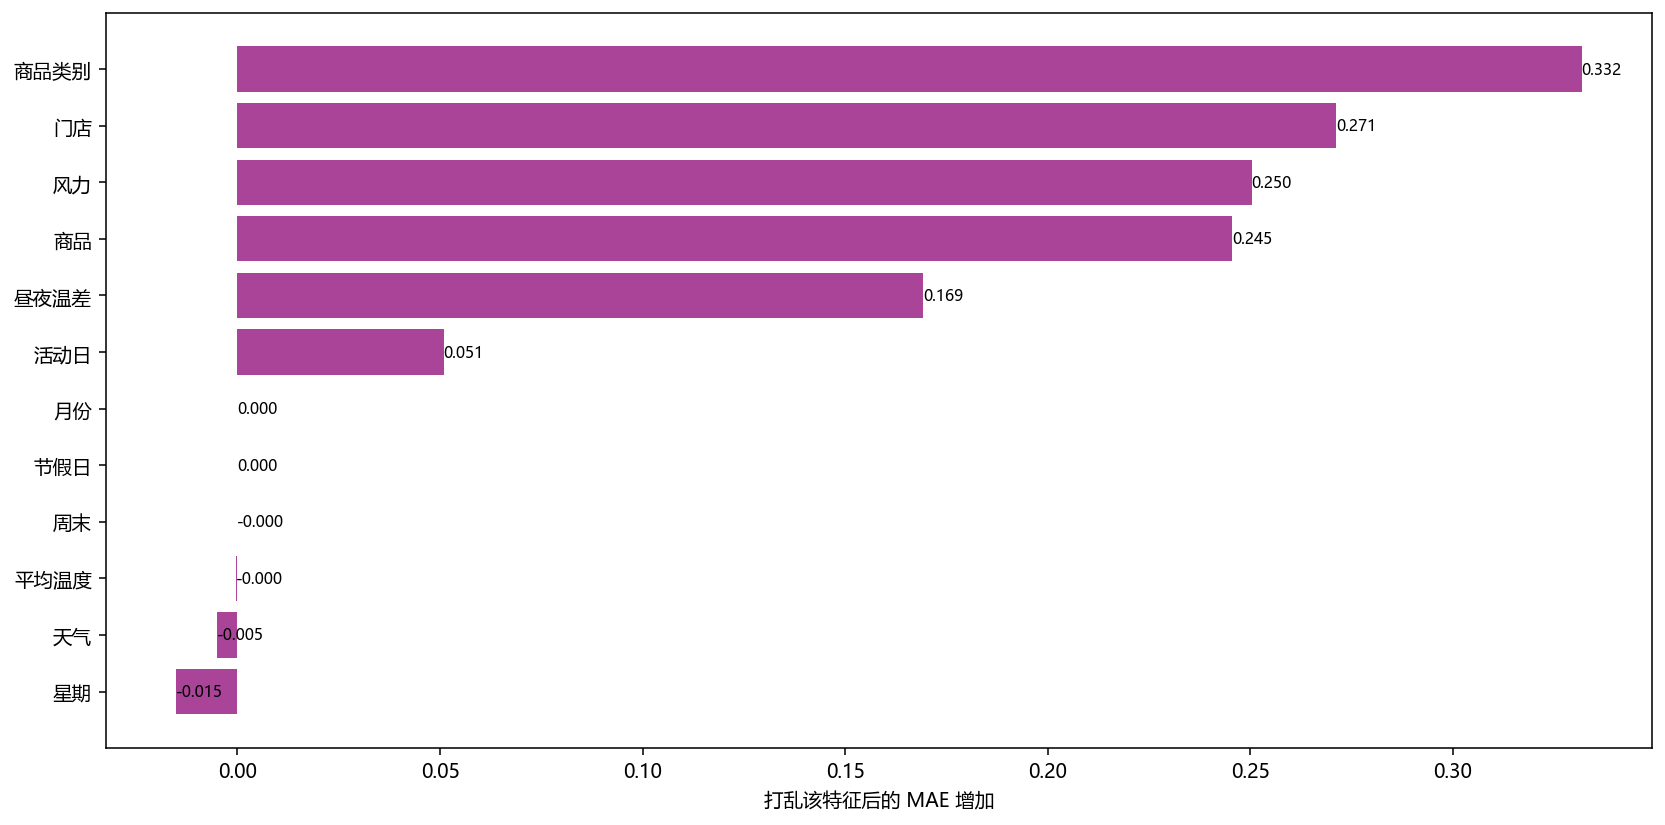
\includegraphics[width=0.82\textwidth]{q3_random_forest_permutation_importance.png}
\caption{随机森林置换重要性，用于展示非线性模型中的预测贡献}
\label{fig:q3_rf}
\end{figure}

\subsection{问题三结果}

描述性统计显示，不同天气、节假日、周末和活动日下的平均销量存在差异，但这些差异可能与门店、商品、星期和月份同时相关。固定效应回归和稳健性检查表明，活动日变量与销量上升之间的统计关联相对更稳定；天气变量存在一定关联，但细分天气类别受样本量限制；节假日和周末与星期效应、月份季节性重叠，结论应作为辅助。本文不分析湿度，因为附件中没有湿度字段。

\section{问题四：综合预测模型与严格递推验证}

问题四需要在门店--商品粒度上进行综合预测。设 $y_{s,p,t}$ 表示门店 $s$、商品 $p$ 在日期 $t$ 的正向销量，综合模型的特征包括历史销量滞后项、滚动均值、日历变量、门店、商品、类别和外部变量。

\subsection{综合模型构造}

综合 Ridge 的特征包括滞后销量、滚动均值、星期、月份、是否周末、门店、商品、类别、天气、节假日和活动日。模型可写为
\begin{equation}
\hat y_{s,p,t}=f(Lag_{s,p,t},Roll_{s,p,t},Cal_t,Store_s,Product_p,Category_p,External_t).
\end{equation}
其中，$Lag$ 包括 \texttt{lag\_1}、\texttt{lag\_7}、\texttt{lag\_14}，$Roll$ 包括 \texttt{rolling\_mean\_7} 和 \texttt{rolling\_mean\_14}。Ridge 回归通过 $L_2$ 正则化缓解多重共线性，适合在保留线性可解释性的同时融合多类特征 \cite{hoerl1970ridge}。随机森林和其他树模型只作为补充比较，不作为论文主模型。

\subsection{严格 7 日递推验证}

信息泄露专项检查 \path{outputs/q4_information_leakage_review.md} 指出：原日滚动验证没有当天销量直接进入当天特征，但验证窗口后续日期的 \texttt{lag\_1} 和滚动均值会使用窗口内前几天真实销量。因此，问题四以 \path{outputs/q4_recursive_7day_model_comparison.md} 中的严格 7 日递推验证作为主口径。

严格递推验证窗口见表 \ref{tab:q4_windows}。每个窗口只使用窗口起点以前的真实历史销量训练模型；窗口内第 2 至第 7 天若需要滞后或滚动特征，则使用前面已经预测出的销量，而不使用窗口内真实销量。

\begin{table}[H]
\centering
\caption{问题四严格 7 日递推验证窗口}
\label{tab:q4_windows}
\begin{tabular}{ccc}
\toprule
窗口起点 & 窗口终点 & 长度 \\
\midrule
2022-03-01 & 2022-03-07 & 7 \\
2022-03-08 & 2022-03-14 & 7 \\
2022-03-15 & 2022-03-21 & 7 \\
2022-03-22 & 2022-03-28 & 7 \\
\bottomrule
\end{tabular}
\end{table}

严格递推下，门店--商品层级误差见表 \ref{tab:q4_metrics}。

\begin{table}[H]
\centering
\caption{问题四严格 7 日递推主粒度误差比较}
\label{tab:q4_metrics}
\begin{tabular}{lrrr}
\toprule
模型 & MAE & RMSE & WAPE \\
\midrule
问题一门店--商品简单指数平滑 & 1.816 & 3.772 & 76.35\% \\
综合 Ridge 回归 & 1.824 & 3.702 & 76.68\% \\
14 日滚动均值基准模型 & 1.847 & 3.819 & 77.66\% \\
7 日移动平均基准模型 & 1.865 & 3.797 & 78.43\% \\
综合随机森林 & 1.988 & 4.842 & 83.60\% \\
\bottomrule
\end{tabular}
\end{table}

在严格 7 日递推验证口径下，综合 Ridge 模型相较部分基准模型仍具有竞争力，但未超过问题一简单指数平滑模型。其主要价值在于统一融合门店、商品、类别、历史销量和外部因素，为多因素解释和情景预测提供一致框架。本文不作全局最优或显著提升的夸大表述。

\subsection{未来 7 天预测与整数化}

未来 7 天天气、温度、风力和活动日没有附件真实观测，最终预测使用历史同期参考情景；清明节日历按 2022-04-03 至 2022-04-05 为节假日、2022-04-02 为调休上班日处理。因此，最终预测为给定外部变量情景下的条件预测。

\begin{figure}[H]
\centering
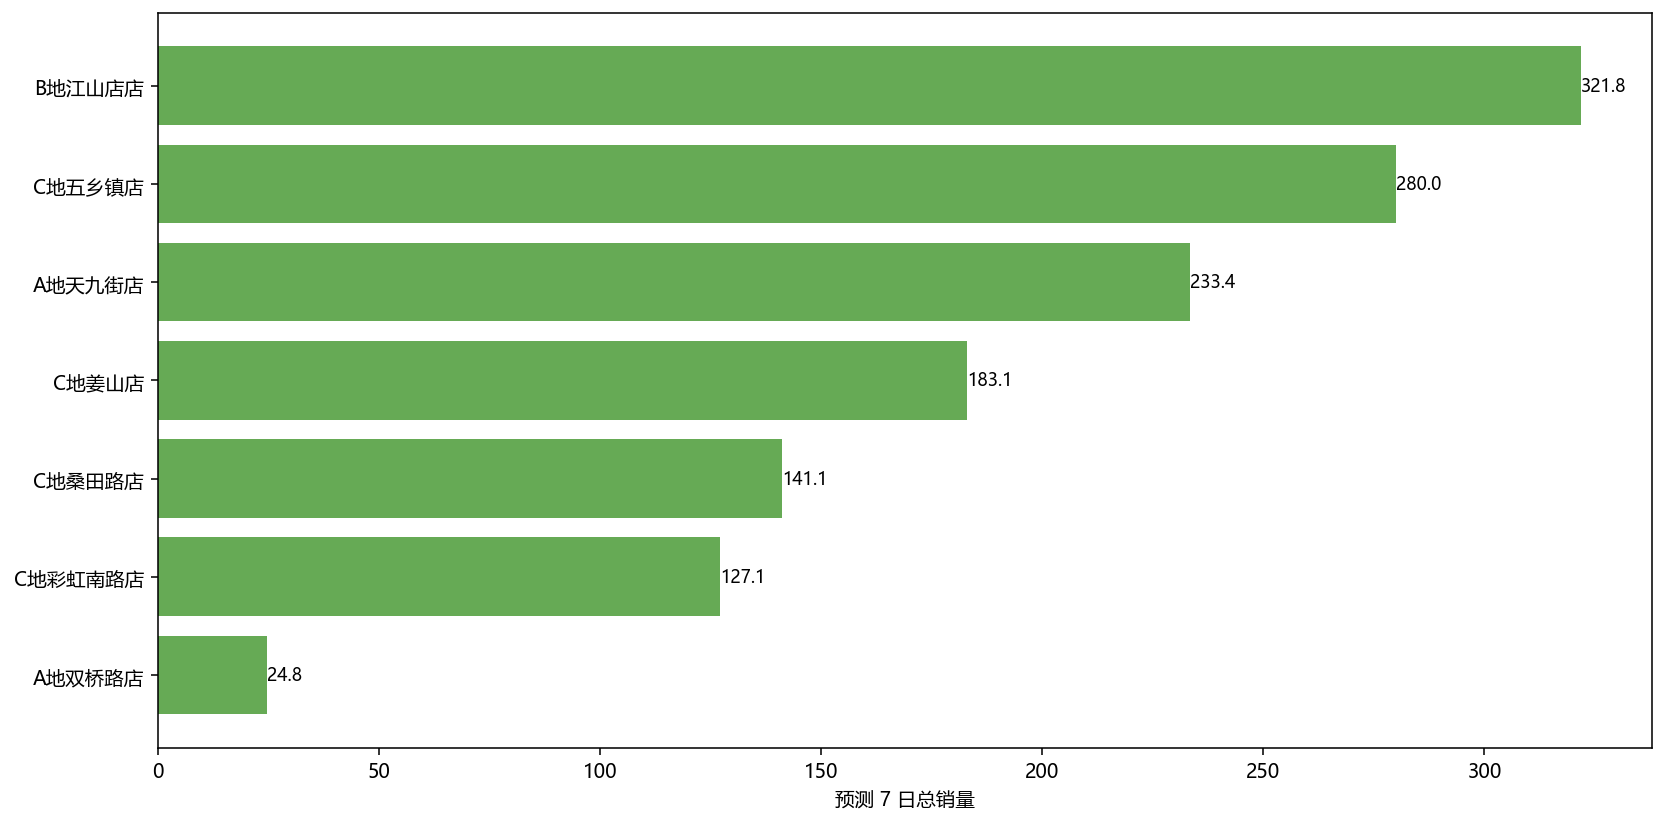
\includegraphics[width=0.85\textwidth]{q4_store_forecast_7day_total.png}
\caption{未来 7 天门店预测总量，用于展示综合模型在门店层面的预测结果}
\label{fig:q4_store_forecast}
\end{figure}

\begin{figure}[H]
\centering
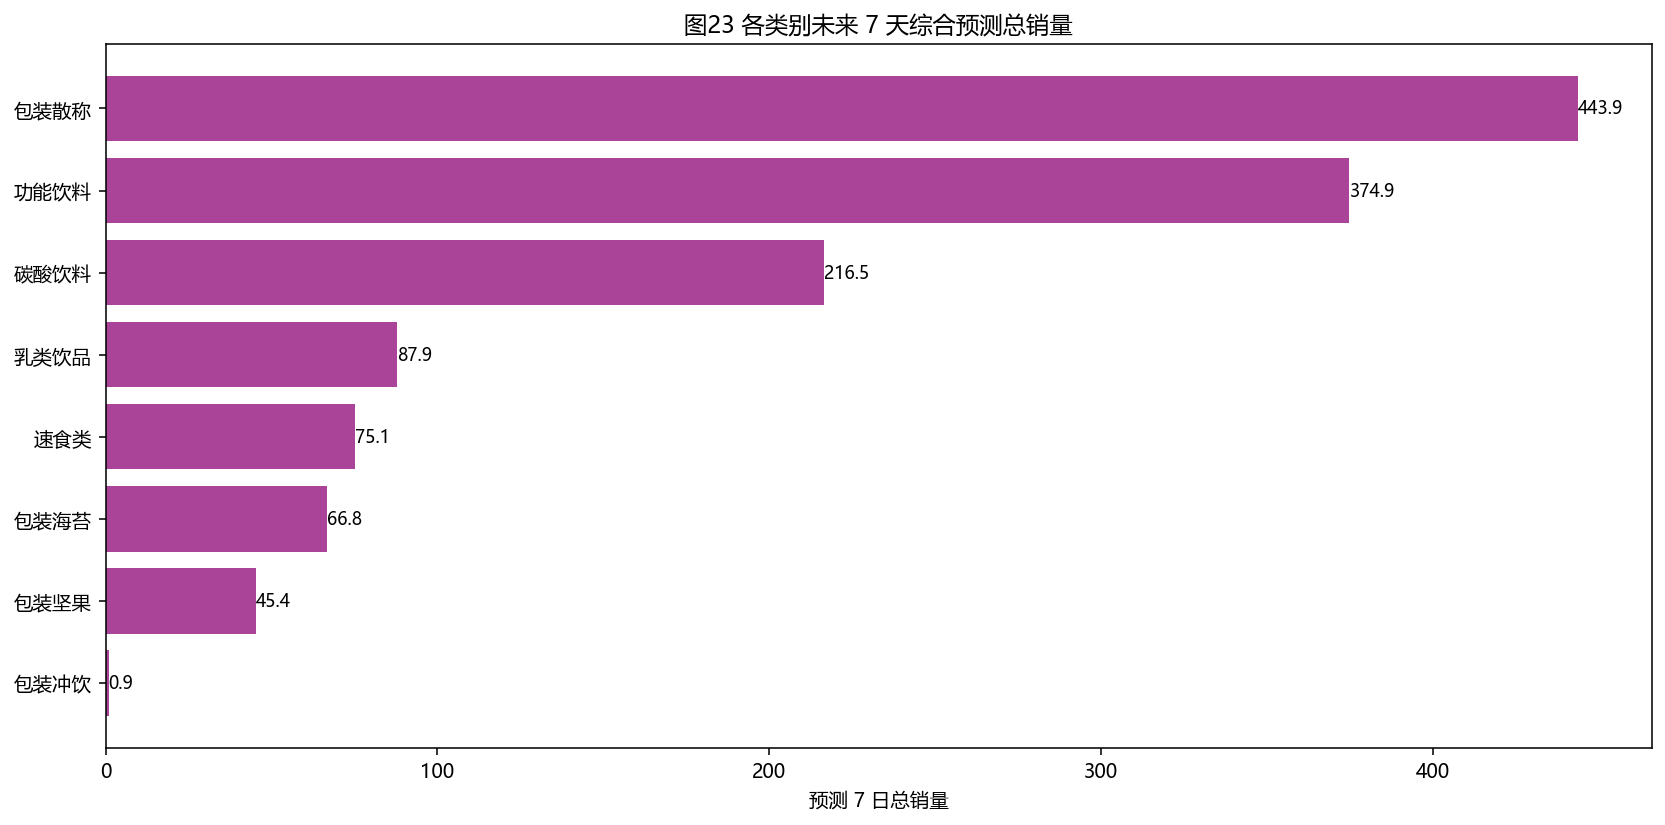
\includegraphics[width=0.85\textwidth]{q4_category_forecast_7day_total.png}
\caption{未来 7 天类别预测总量，用于展示综合模型在类别层面的预测结果}
\label{fig:q4_category_forecast}
\end{figure}

未来 7 天综合 Ridge 条件预测中，各门店预测总销量最高的是 B地江山店店 321.801，其次为 C地五乡镇店 279.972 和 A地天九街店 233.438；各类别预测最高的是包装散称 443.881，其次为功能饮料 374.886 和碳酸饮料 216.494。完整门店--商品--日期小数预测表见 \path{outputs/final_7day_forecast.csv}。

由于实际销量以件数计，提交展示时对模型预测值进行非负约束和四舍五入整数化处理：预测值小于 0 的先置为 0，其余按四舍五入转为整数；原始小数预测结果仍作为模型连续输出保留。整数化预测表为 \path{outputs/final_7day_forecast_integer.csv}。小数预测表 7 天预测总量为 1311.294，整数化后 7 天预测总量为 1309。

\subsection{误差诊断与情景敏感性}

天气敏感性检验 \path{outputs/q4_weather_sensitivity_report.md} 显示，完整外部变量 Ridge 的严格递推 WAPE 为 76.68\%，去除天气变量 Ridge 为 77.73\%，历史同期天气情景 Ridge 为 76.57\%。因此，天气变量可作为补充情景特征，但不能写成稳定因果因素。

误差诊断 \path{outputs/q4_error_diagnosis_report.md} 显示，综合 Ridge 在门店 A地双桥路店、低销量商品和样本不足的活动日场景误差较大；间歇性需求审查 \path{outputs/intermittent_demand_review.md} 显示，76 条门店--商品序列中有 54 条零销量比例不低于 50\%，解释了门店--商品层级 WAPE 较高的原因。间歇性需求建模思想可参考 Croston 方法 \cite{croston1972intermittent}，但本文不将其作为主模型。

\begin{figure}[H]
\centering
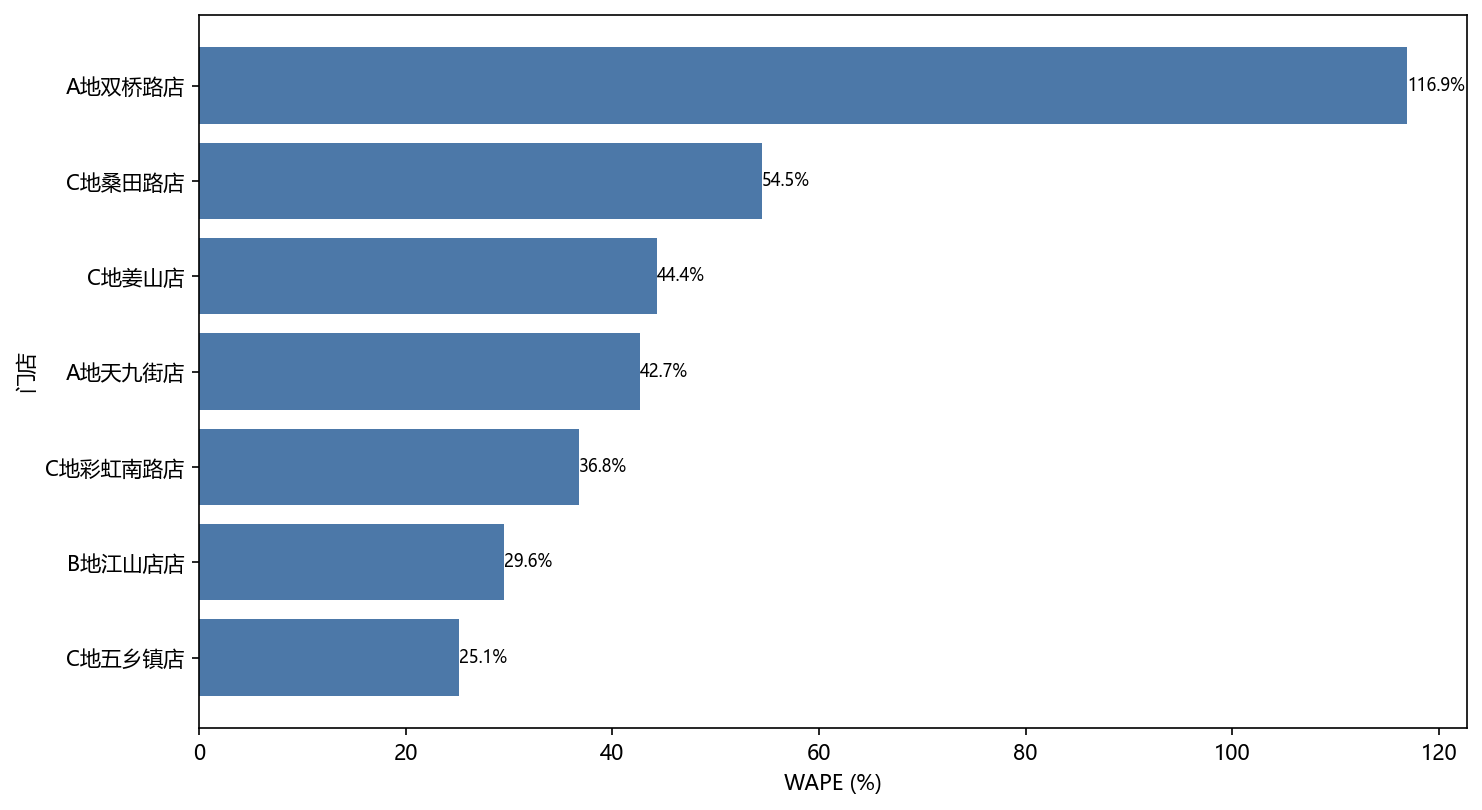
\includegraphics[width=0.85\textwidth]{q4_error_by_store_bar.png}
\caption{门店误差诊断，用于定位严格递推验证下误差较高的门店}
\label{fig:q4_error_store}
\end{figure}

\begin{figure}[H]
\centering
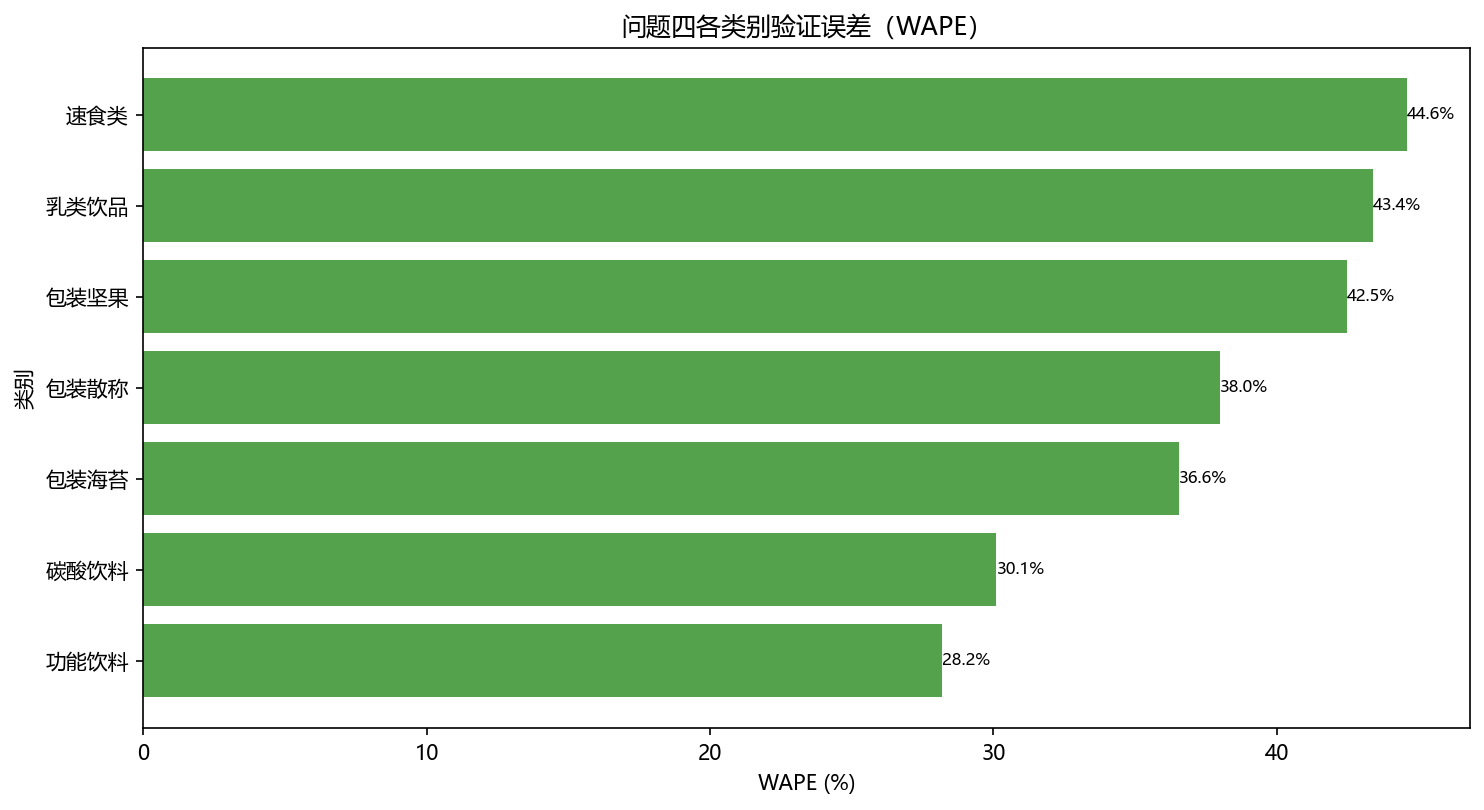
\includegraphics[width=0.85\textwidth]{q4_error_by_category_bar.png}
\caption{类别误差诊断，用于定位严格递推验证下误差较高的类别}
\label{fig:q4_error_category}
\end{figure}

\begin{figure}[H]
\centering
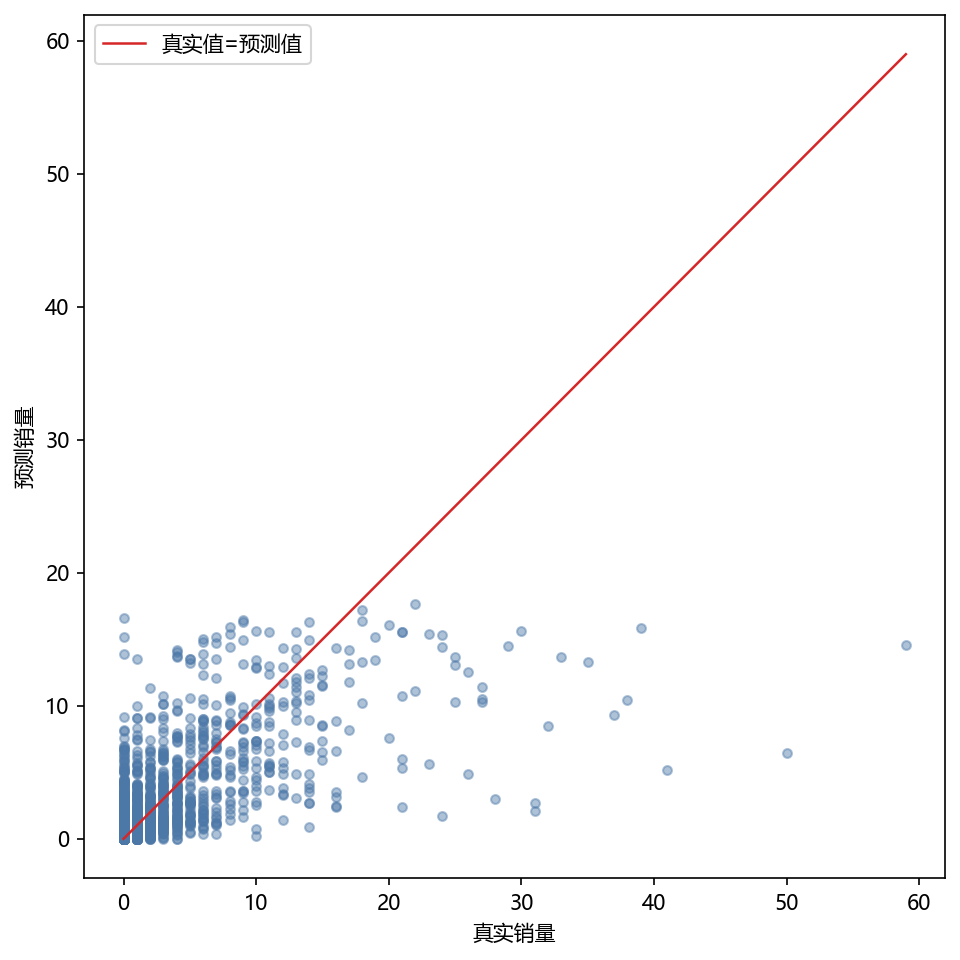
\includegraphics[width=0.82\textwidth]{q4_actual_vs_predicted_scatter.png}
\caption{严格递推验证真实值与预测值散点，用于检查预测值与真实值的对应关系}
\label{fig:q4_scatter}
\end{figure}

\section{模型评价}

\subsection{误差指标}

本文主要采用 MAE、RMSE 和 WAPE 评价预测误差：
\begin{equation}
MAE=\frac{1}{n}\sum_{i=1}^{n}|y_i-\hat y_i|,
\end{equation}
\begin{equation}
RMSE=\sqrt{\frac{1}{n}\sum_{i=1}^{n}(y_i-\hat y_i)^2},
\end{equation}
\begin{equation}
WAPE=\frac{\sum_{i=1}^{n}|y_i-\hat y_i|}{\sum_{i=1}^{n}|y_i|}.
\end{equation}
MAE 表示平均绝对偏差，便于解释平均误差规模；RMSE 对大误差更敏感，适合检查极端预测偏差；WAPE 用总绝对误差除以总实际销量，适合本题中不同门店和商品销量规模差异较大的情况。对于真实销量为 0 的类别或商品，WAPE 无法定义，需要结合 MAE 和预测合计单独说明。

\subsection{分问题评价}

问题一中，日滚动验证结果显示，门店层面移动平均(7日) WAPE=37.49\%，商品层面简单指数平滑 WAPE=38.14\%，门店--商品层面简单指数平滑 WAPE=74.95\%。补充的 7 日窗口总量验证表明，原问题一主方案在商品层面 WAPE=21.51\%，门店层面 WAPE=22.12\%，门店--商品层面 WAPE=43.06\%。因此，问题一采用简单可解释模型作为基础预测框架。

问题二中，类别聚合后直接预测 + 简单指数平滑的 WAPE=34.74\%，略优于单品预测后按类别加总的 WAPE=34.83\%。销量规模分组 WAPE=24.24\%，相关性聚类 WAPE=31.02\%，但二者不直接回答“同类零食类别预测”要求，因此只作为补充，不作为主方案。

问题三中，合并天气、对数销量和历史控制固定效应回归的验证 WAPE=84.53\%，优于原详细天气固定效应回归的 WAPE=88.09\%。随机森林 grouped weather + history 的 WAPE=84.66\%，可作为预测贡献补充，但不提供清晰方向，也不用于识别因果效应。问题三主结论应写成“条件统计关联”。

问题四中，严格 7 日递推验证是主评价口径。该口径下，问题一门店--商品简单指数平滑 WAPE=76.35\%，综合 Ridge WAPE=76.68\%，14 日滚动均值基准模型 WAPE=77.66\%，7 日移动平均基准模型 WAPE=78.43\%。综合 Ridge 优于问题四内部基准模型，但未超过问题一强基准模型。因此，综合模型的作用主要是融合前三问信息并提供统一解释框架。进一步的低销量鲁棒性检验显示，低销量序列使用指数平滑、常规序列使用综合 Ridge 的混合策略 WAPE=75.85\%，相对问题一强基准降低 0.49 个百分点；该结果说明细粒度稀疏需求需要分层处理，但改进幅度仍应谨慎解释。附加比较还考察了不同低销量阈值、近 28 日均值兜底和层级比例校准；虽然近 28 日均值方案在同一验证集上 WAPE=74.95\%，但留一窗口选模平均改善仅 0.19 个百分点，稳定性证据不足，故不作为正文主预测口径。

\subsection{不确定性}

不确定性主要来自四类来源。第一，未来天气和活动日采用历史同期情景，若实际天气或促销安排偏离该情景，最终预测会变化。第二，低销量门店--商品序列存在大量零销量，当前混合策略下低销量序列整体 WAPE 约为 122.53\%，少量绝对误差即可被低销量分母放大；混合策略虽有所改善，但并未消除稀疏需求带来的不确定性。第三，部分稀有天气样本天数较少，例如雨夹雪、暴雨等，不能把其系数作为稳定主结论。第四，严格递推验证只有 4 个完整 7 日窗口，模型选择结论仍需谨慎。

为辅助解释最终点预测，本文基于当前混合策略在 4 个严格 7 日递推验证窗口上的 7 日聚合残差构造经验区间。对每个门店、商品或类别，先计算“真实 7 日销量减预测 7 日销量”的残差，再取历史残差的 10\% 和 90\% 分位数加到未来点预测上，形成经验 80\% 残差区间。该区间不是严格置信区间，主要反映历史递推误差下的不确定性范围。门店级结果见图 \ref{fig:q4_store_interval}。

\begin{figure}[H]
\centering
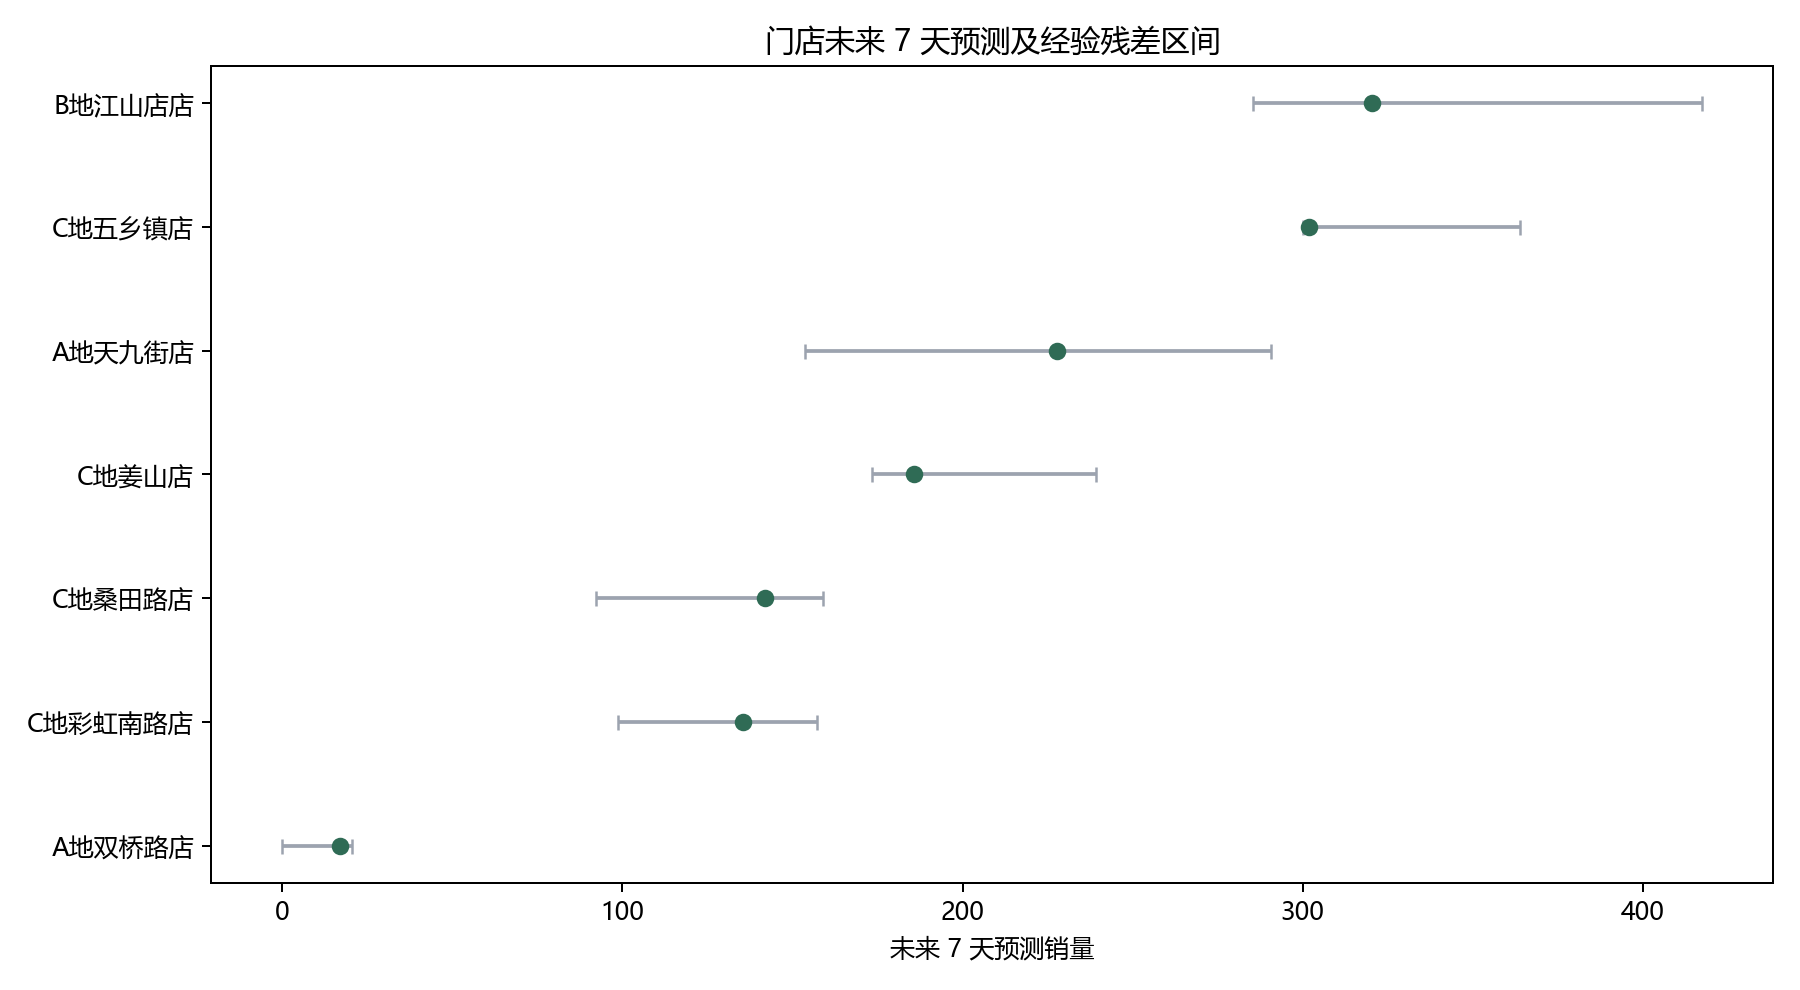
\includegraphics[width=0.86\textwidth]{final_forecast_interval_by_store.png}
\caption{基于严格递推残差的门店未来 7 天经验预测区间}
\label{fig:q4_store_interval}
\end{figure}

\section{优缺点分析与结论}

\subsection{模型优点}

本文模型具有以下优点：
\begin{enumerate}
  \item 数据口径清晰，区分正向销量、净销量和负向调整。
  \item 模型与题目四问一一对应，形成门店、商品、类别和门店--商品的分层预测框架。
  \item 主模型优先采用移动平均、同星期均值、指数平滑和固定效应回归，公式简单、可解释、易复现。
  \item 对综合模型进行了信息泄露审查，并以严格 7 日递推验证作为主口径。
  \item 对外部变量和商品关联均设置了证据边界，没有把相关性写成因果性。
\end{enumerate}

\subsection{模型局限}

本文模型存在以下局限。第一，门店--商品粒度存在大量零销量与间歇性需求，76 条序列中 54 条零销量比例不低于 50\%，构成细粒度预测的结构性误差上限；WAPE 因低销量分母放大而偏高，混合策略只能部分缓解。第二，未来真实天气与促销安排不可得，含外部变量预测依赖历史同期情景，属于条件预测。第三，附件缺少顾客购物篮、价格、库存与陈列信息，无法识别商品互补/替代和促销因果效应，问题二、问题三结论均限于统计关联。第四，严格递推验证仅含 4 个完整 7 日窗口，统计功效有限，显著性检验和稳定性判断应谨慎推广。

\subsection{模型推广}

该框架可以推广到更多门店和更多品类。若新增门店或商品，只需按日期--门店--商品构造同样的日销量面板，并在门店、商品和类别层级分别保留可解释基准模型，再用严格 7 日递推检验综合模型是否真正优于强基准。若后续取得价格、库存、陈列位置和促销力度等字段，可以把这些变量并入 $x_{s,p,t}$，在预测任务中作为外部特征，在解释任务中则需继续区分统计关联和因果效应；若存在促销随机实验或明确的政策切换，再考虑因果识别方法。对零销量比例较高的商品，可进一步引入 Croston 族或 Syntetos--Boylan Approximation 等间歇需求模型 \cite{syntetos2005accuracy}，但仍应与简单指数平滑、移动平均等基准模型在同一验证口径下比较。

\subsection{结论}

本文完成了休闲零食连锁店商品销量预测的四问建模。问题一保留移动平均、同星期均值和简单指数平滑，建立了门店、商品和门店--商品的基础预测；问题二以附件类别字段整合同类零食，商品相关性分析作为同步波动证据，类别预测主方案为类别聚合后直接预测；问题三采用合并天气、对数销量和历史控制固定效应回归，得到外部变量与销量之间的条件统计关联；问题四采用综合 Ridge 模型融合前三问信息，并用严格 7 日递推验证检验未来 7 天预测能力。

本文围绕销量预测四问，建立了由简单基准到综合融合、口径逐级衔接的分层框架。最重要的发现有两点：其一，在本题数据下，简单可解释模型在严格递推口径下与复杂模型相当，复杂度的边际误差收益受限；其二，门店--商品层高误差主要由间歇需求结构决定，而非单纯建模能力不足。问题四综合 Ridge 虽然能整合前三问信息，但在严格 7 日递推主粒度下未超过问题一门店--商品简单指数平滑强基准模型。进一步的低销量鲁棒性检验表明，对低销量组合采用指数平滑、对常规组合采用综合 Ridge 的混合策略在严格递推主粒度上 WAPE=75.85\%，相对简单基准下降 0.49 个百分点，但统计检验未支持“显著改进”。基于此，本文以“低销量序列指数平滑 + 常规序列综合 Ridge”的混合策略生成未来 7 天条件预测；所有层级预测经统一整数化后由门店--商品--日期最细粒度求和，保证门店、商品、类别与总计汇总一致。整数化预测总量为 1328，汇总表见附录 D，完整明细可作为电子附件提交。


\bibliographystyle{plain}
\bibliography{references}

\appendix
\section{附录}

\subsection{代码文件清单与复现顺序}

项目代码、数据处理说明和复现入口已整理在 GitHub 仓库：
\url{https://github.com/tyloo-knife/snack-sales-forecast}。

主要代码文件如下：

\begin{itemize}
  \item 数据读取与清洗：\path{src/data_loader.py}、\path{src/preprocessing.py}
  \item 特征工程：\path{src/features.py}
  \item 问题二分析：\path{src/stage3_q2_analysis.py}
  \item 问题三分析：\path{src/stage4_q3_analysis.py}
  \item 问题四综合模型：\path{src/stage5_q4_analysis.py}
  \item 严格递推验证：\path{src/stage5_q4_recursive_validation.py}
  \item 问题四误差诊断：\path{src/stage5_q4_error_diagnosis.py}
  \item 天气敏感性分析：\path{src/stage5_q4_weather_sensitivity.py}
  \item 间歇性需求审查：\path{src/intermittent_demand_review.py}
\end{itemize}

建议复现顺序如下：

\begin{enumerate}
  \item 安装依赖：在仓库根目录运行 \path{python -m pip install -r requirements.txt}。
  \item 确认原始附件位于 \path{data/raw/}，处理后数据位于 \path{data/processed/}。
  \item 运行问题二脚本：\path{python src/stage3_q2_analysis.py}。
  \item 运行问题三脚本：\path{python src/stage4_q3_analysis.py}。
  \item 运行问题四综合模型：\path{python src/stage5_q4_analysis.py}。
  \item 运行严格 7 日递推验证：\path{python src/stage5_q4_recursive_validation.py}。
  \item 运行误差诊断、天气敏感性和间歇性需求检查：依次执行 \path{src/stage5_q4_error_diagnosis.py}、\path{src/stage5_q4_weather_sensitivity.py}、\path{src/intermittent_demand_review.py}。
\end{enumerate}

\subsection{主要结果文件}

\begin{itemize}
  \item 数据检查：\path{outputs/stage1_data_inspection_report.md}
  \item 问题一报告：\path{outputs/stage2_q1_modeling_report.md}
  \item 问题二报告：\path{outputs/stage3_q2_relationship_report.md}
  \item 问题三报告：\path{outputs/stage4_q3_factor_analysis_report.md}
  \item 问题四报告：\path{outputs/stage5_q4_final_model_report.md}
  \item 信息泄露审查：\path{outputs/q4_information_leakage_review.md}
  \item 严格递推验证：\path{outputs/q4_recursive_7day_model_comparison.md}
  \item 误差诊断：\path{outputs/q4_error_diagnosis_report.md}
  \item 天气敏感性检验：\path{outputs/q4_weather_sensitivity_report.md}
  \item 间歇性需求审查：\path{outputs/intermittent_demand_review.md}
  \item 实验结果摘要：\path{RESULT_LOG.md}
  \item 小数预测表：\path{outputs/final_7day_forecast.csv}
  \item 整数预测表：\path{outputs/final_7day_forecast_integer.csv}
\end{itemize}

\subsection{辅助工具使用说明}

辅助工具主要用于代码排错、文档一致性检查和 LaTeX 排版整理。字段解释、负销量口径、模型取舍、问题四验证口径和最终结论均由小组成员依据附件数据和实验结果确认。若课程或竞赛要求单独披露辅助工具使用情况，可参考 \path{submission/ai_usage_record.md}。


\end{document}
